%==============================================================================
%== LLM Software Development Poster (1.2m x 0.9m) — 순서 변경판 ===============
%==============================================================================
\documentclass[final]{beamer}
\usepackage[orientation=portrait,size=custom,width=90,height=120,scale=1.1]{beamerposter}

% --- [중요] 폰트 및 언어 설정 (XeLaTeX 전용) ---
\usepackage{xeCJK}
% Fandol: TeXLive/MiKTeX 기본 번들 중국어 폰트 → 로컬·Overleaf 모두 동일하게 작동.
% beamer는 sans 기반이므로 main/sans 모두 흑체(FandolHei)로 지정.
\setCJKmainfont{FandolHei-Regular.otf}[BoldFont=FandolHei-Bold.otf]
\setCJKsansfont{FandolHei-Regular.otf}[BoldFont=FandolHei-Bold.otf]
\setCJKmonofont{FandolFang-Regular.otf}
\linespread{0.95} 

\usepackage{tikz}
\usetikzlibrary{shapes, arrows, positioning, calc}
\usepackage{multicol}
\usepackage{booktabs}

% --- 이미지 경로: 로컬(fig4poster/)과 Overleaf(root, ./) 양쪽 모두 탐색 ---
\graphicspath{{fig4poster/}{fig4poster/microscope/}{fig4poster/note_editor/}{fig4poster/macro/}{microscope/}{note_editor/}{macro/}{./}}

% 색상 정의
\definecolor{posterpurple}{HTML}{8A4BA3}
\definecolor{posternavy}{HTML}{322659}
\definecolor{blocktitlebg}{HTML}{9B72CF} % 블록 제목 배경: 연한 보라

%==============================================================================
% 헤더 디자인
%==============================================================================
\setbeamertemplate{headline}{
  \begin{beamercolorbox}[wd=\paperwidth]{headline}
    \begin{tikzpicture}[remember picture, overlay]
      \node[anchor=north west, inner sep=0pt] at (current page.north west) {
        
\includegraphics[width=\paperwidth, height=10cm]{header.png}
      };
      \node[anchor=center, text=white] at ($(current page.north)+(0,-3.6cm)$) {
        \fontsize{76pt}{64pt}\selectfont \textbf{大模型驱动的软件开发 课程成果展示}
      };
      \node[anchor=center, text=white] at ($(current page.north)+(0,-7cm)$) {
        \fontsize{58pt}{44pt}\selectfont \textbf{GraphNode -- Your next second Brain}
      };
    \end{tikzpicture}
    \vspace{9cm} % 헤더와 본문 사이 간격 (줄일수록 본문이 위로 올라옴)
  \end{beamercolorbox}
}

%==============================================================================
% 푸터 디자인
%==============================================================================
\setbeamertemplate{footline}{
  \begin{beamercolorbox}[wd=\paperwidth]{footline}
    \begin{tikzpicture}[remember picture, overlay]
      \node[anchor=south west, inner sep=0pt] at (current page.south west) {
        
\includegraphics[width=\paperwidth, height=3cm]{footer.png}
      };
      \node[anchor=center, text=white] at ($(current page.south)+(0,1.5cm)$) {
        \fontsize{28pt}{34pt}\selectfont \textbf{联系人：韩佑硕 \quad 邮箱：hanys21@mails.tsinghua.edu.cn \quad 2026 春季学期}
      };
    \end{tikzpicture}
    \vspace{3cm}
  \end{beamercolorbox}
}
\setbeamertemplate{navigation symbols}{}

%==============================================================================
% 배경: 옅은 knowledge-graph 노드 패턴
%==============================================================================
\setbeamertemplate{background}{%
  \begin{tikzpicture}[remember picture, overlay]
    \begin{scope}[opacity=0.08]
      \foreach \x/\y/\r in {%
        7/112/0.8, 25/104/0.6, 45/114/0.6, 66/107/0.7, 84/112/0.5,
        14/86/0.6, 36/92/0.9, 58/84/0.6, 80/90/0.7,
        10/58/0.7, 32/64/0.6, 54/56/0.9, 76/62/0.6,
        18/30/0.6, 44/24/0.8, 70/32/0.6, 86/22/0.5, 30/12/0.6}{
        \fill[posterpurple] ($(current page.south west)+(\x,\y)$) circle (\r);
      }
      \foreach \ax/\ay/\bx/\by in {%
        7/112/25/104, 25/104/45/114, 45/114/66/107, 66/107/84/112,
        7/112/14/86, 25/104/36/92, 45/114/36/92, 66/107/58/84, 84/112/80/90,
        14/86/36/92, 36/92/58/84, 58/84/80/90,
        14/86/10/58, 36/92/32/64, 58/84/54/56, 80/90/76/62,
        10/58/32/64, 32/64/54/56, 54/56/76/62,
        10/58/18/30, 32/64/44/24, 54/56/70/32, 76/62/86/22,
        18/30/44/24, 44/24/70/32, 70/32/86/22, 18/30/30/12, 44/24/30/12}{
        \draw[posterpurple, line width=2.2pt]
          ($(current page.south west)+(\ax,\ay)$) -- ($(current page.south west)+(\bx,\by)$);
      }
    \end{scope}
  \end{tikzpicture}%
}

\begin{document}
\begin{frame}[t]

\setbeamerfont{block title}{size=\fontsize{46pt}{54pt}}
\setbeamercolor{block title}{fg=white,bg=blocktitlebg}
\setbeamercolor{block body}{fg=black,bg=}

\begin{columns}[t]

%========================== 왼쪽 단 ==========================
\begin{column}{0.46\paperwidth}
\fontsize{36pt}{46pt}\selectfont

% ---- 1. 问题 & 解决方案 ----
\begin{block}{1. 问题 \& 解决方案}
\textbf{对话的增加, 知识却在流失。} 现代知识工作者每天与 LLM 进行频繁交互，
但产生的深度洞见往往随对话结束而消散，沦为\textbf{碎片化、瞬时性}的信息泡沫。\\[0.2cm]
\textbf{GraphNode} 是一款创新的\textbf{第二大脑（Second Brain）平台}。它能自动分析 AI 对话与笔记，
并将其转化为\textbf{交互式知识图谱}，实现：\textbf{跨平台知识连接}（整合 ChatGPT / Claude / Notion / Obsidian 等）、
\textbf{深度洞察提炼}与\textbf{全流程自动化生成}（无需手动打标）。
\vspace{-0.1cm}\\
\noindent
\begin{minipage}[t]{0.495\linewidth}\vspace{0pt}\centering

\includegraphics[width=\linewidth, height=12cm, keepaspectratio]{problem.jpg}\\[-0.1cm]
{\fontsize{22pt}{28pt}\selectfont 知识碎片化的恶循环}
\end{minipage}\hfill
\begin{minipage}[t]{0.495\linewidth}\vspace{0pt}\centering

\includegraphics[width=\linewidth, height=12cm, keepaspectratio]{solution.jpg}\\[-0.1cm]
{\fontsize{22pt}{28pt}\selectfont 连接为真正的知识资产}
\end{minipage}
\end{block}

% ---- 2. 知识结构化：Macro & Microscope (구 3) ----
\begin{block}{2. 知识结构化：Macro \& Microscope}
\raggedright
\textbf{Macro Graph}：跨用户\textbf{所有}对话/笔记的全局鸟瞰图，三级层次
\textbf{Cluster $\rightarrow$ Sub-cluster $\rightarrow$ Node}，语义相似节点自动连边；\\
配合 \textbf{Graph Summary}（模式识别 / 定制建议）。
\\[-0.4cm]
\noindent
\begin{minipage}[t]{0.62\linewidth}\vspace{0pt}\centering
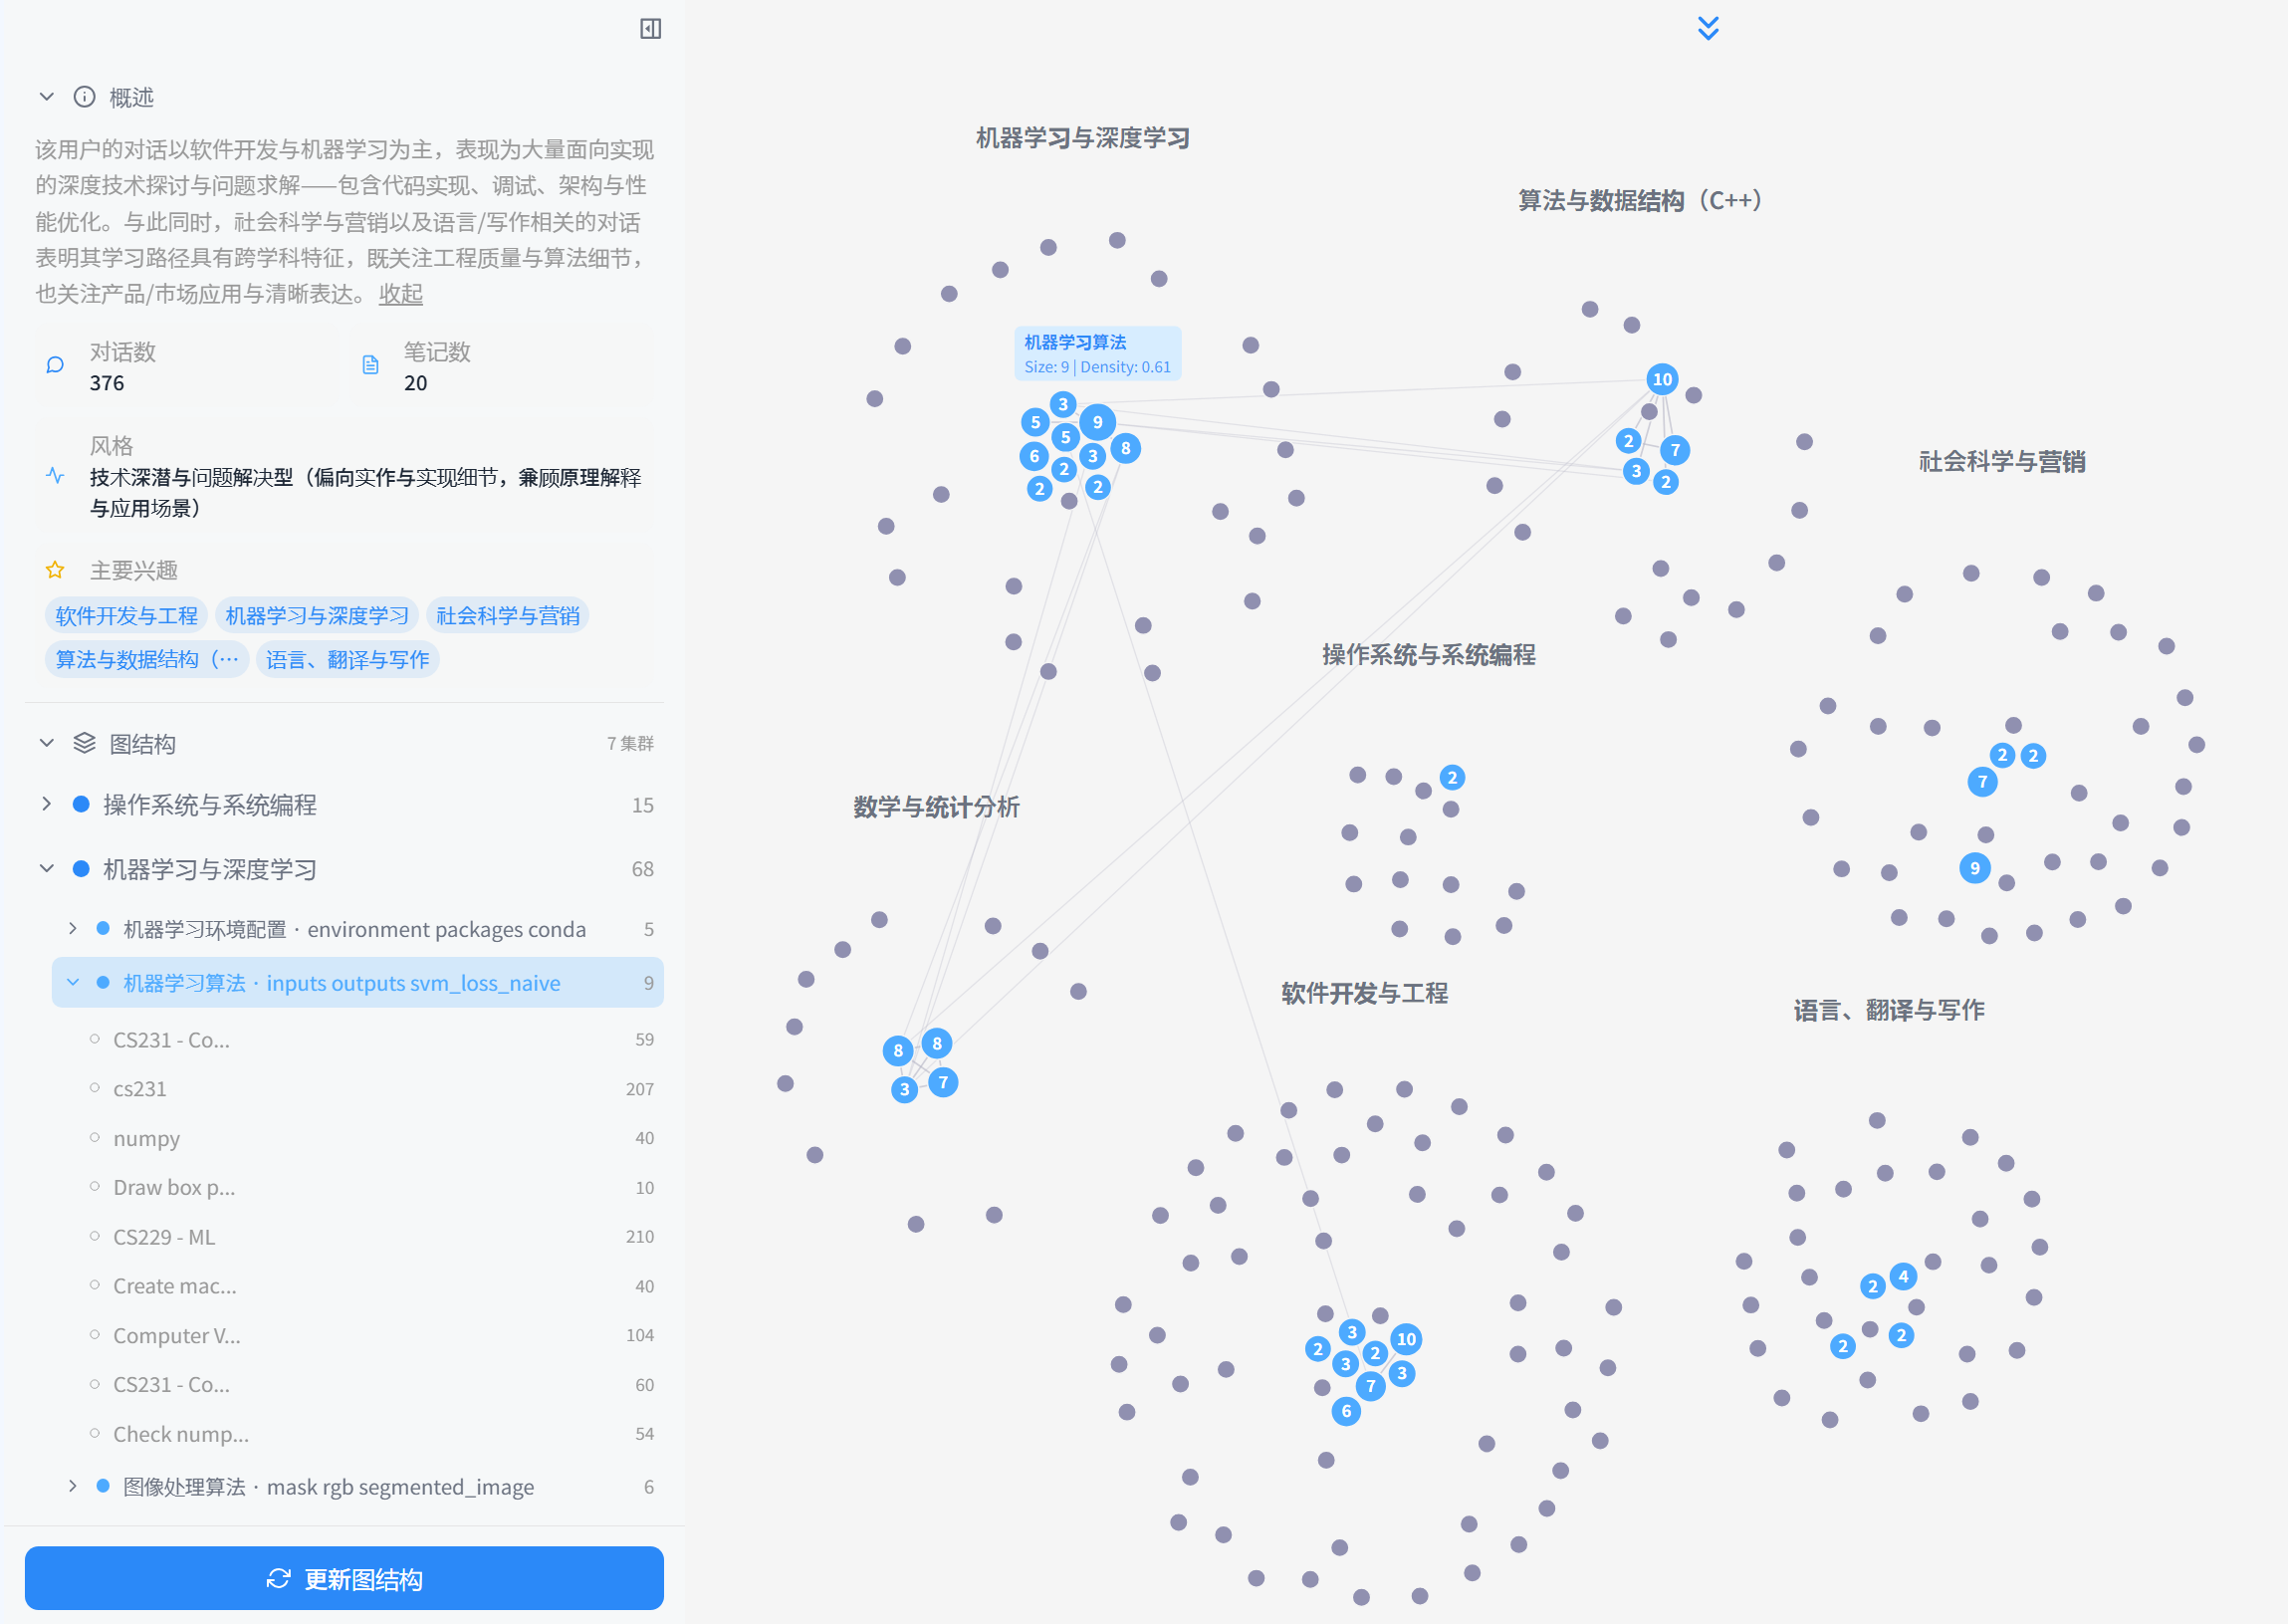
\includegraphics[width=\linewidth, height=14cm, keepaspectratio]{macro_graph.png}\par\vspace{-0.25cm}
{\fontsize{20pt}{26pt}\selectfont Macro Graph}
\end{minipage}\hfill
\begin{minipage}[t]{0.34\linewidth}\vspace{0pt}\centering
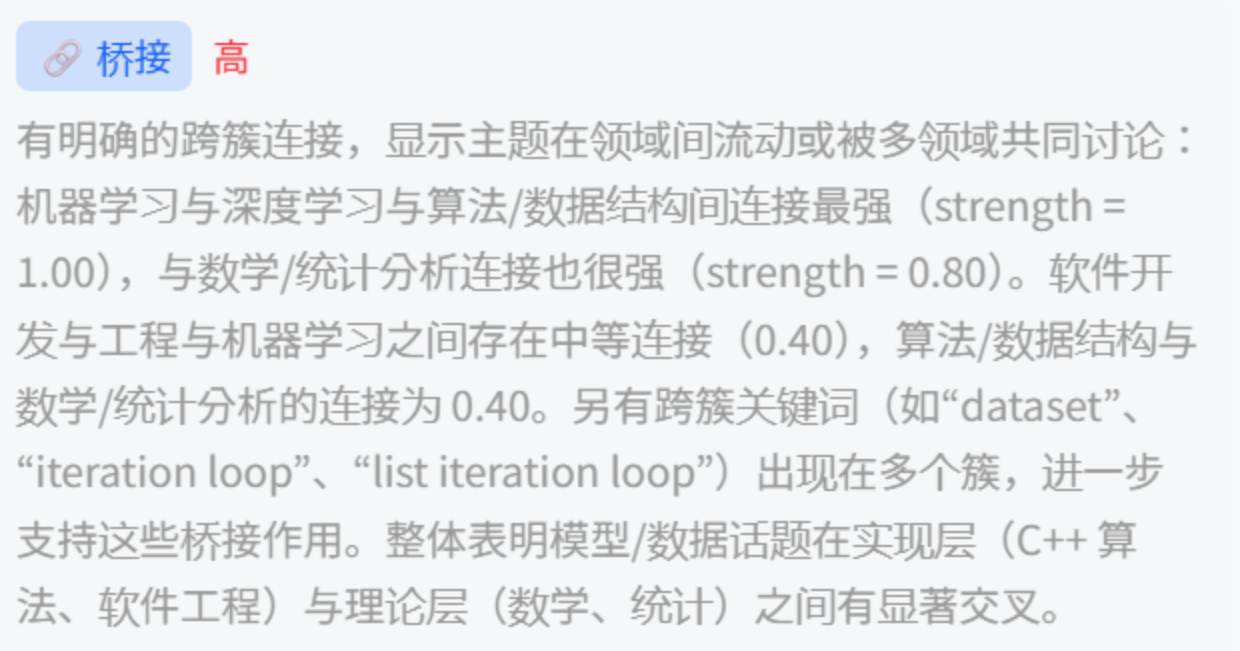
\includegraphics[width=\linewidth, height=7cm, keepaspectratio]{user_patterns.png}\par\vspace{-0.25cm}
{\fontsize{20pt}{26pt}\selectfont 模式识别}\par\medskip

\includegraphics[width=\linewidth, height=7cm, keepaspectratio]{macro_suggestions.png}\par\vspace{-0.25cm}
{\fontsize{20pt}{26pt}\selectfont 定制建议}
\end{minipage}\\
\textbf{Microscope}：聚焦\textbf{单一文档内部}，由LLM提取node与edge生成专属knowledge graph，帮助快速把握一篇文档/对话的整体结构与主旨。两种视图：
\vspace{-0.45cm}\\
\noindent
\begin{minipage}[t]{0.495\linewidth}\vspace{0pt}\centering
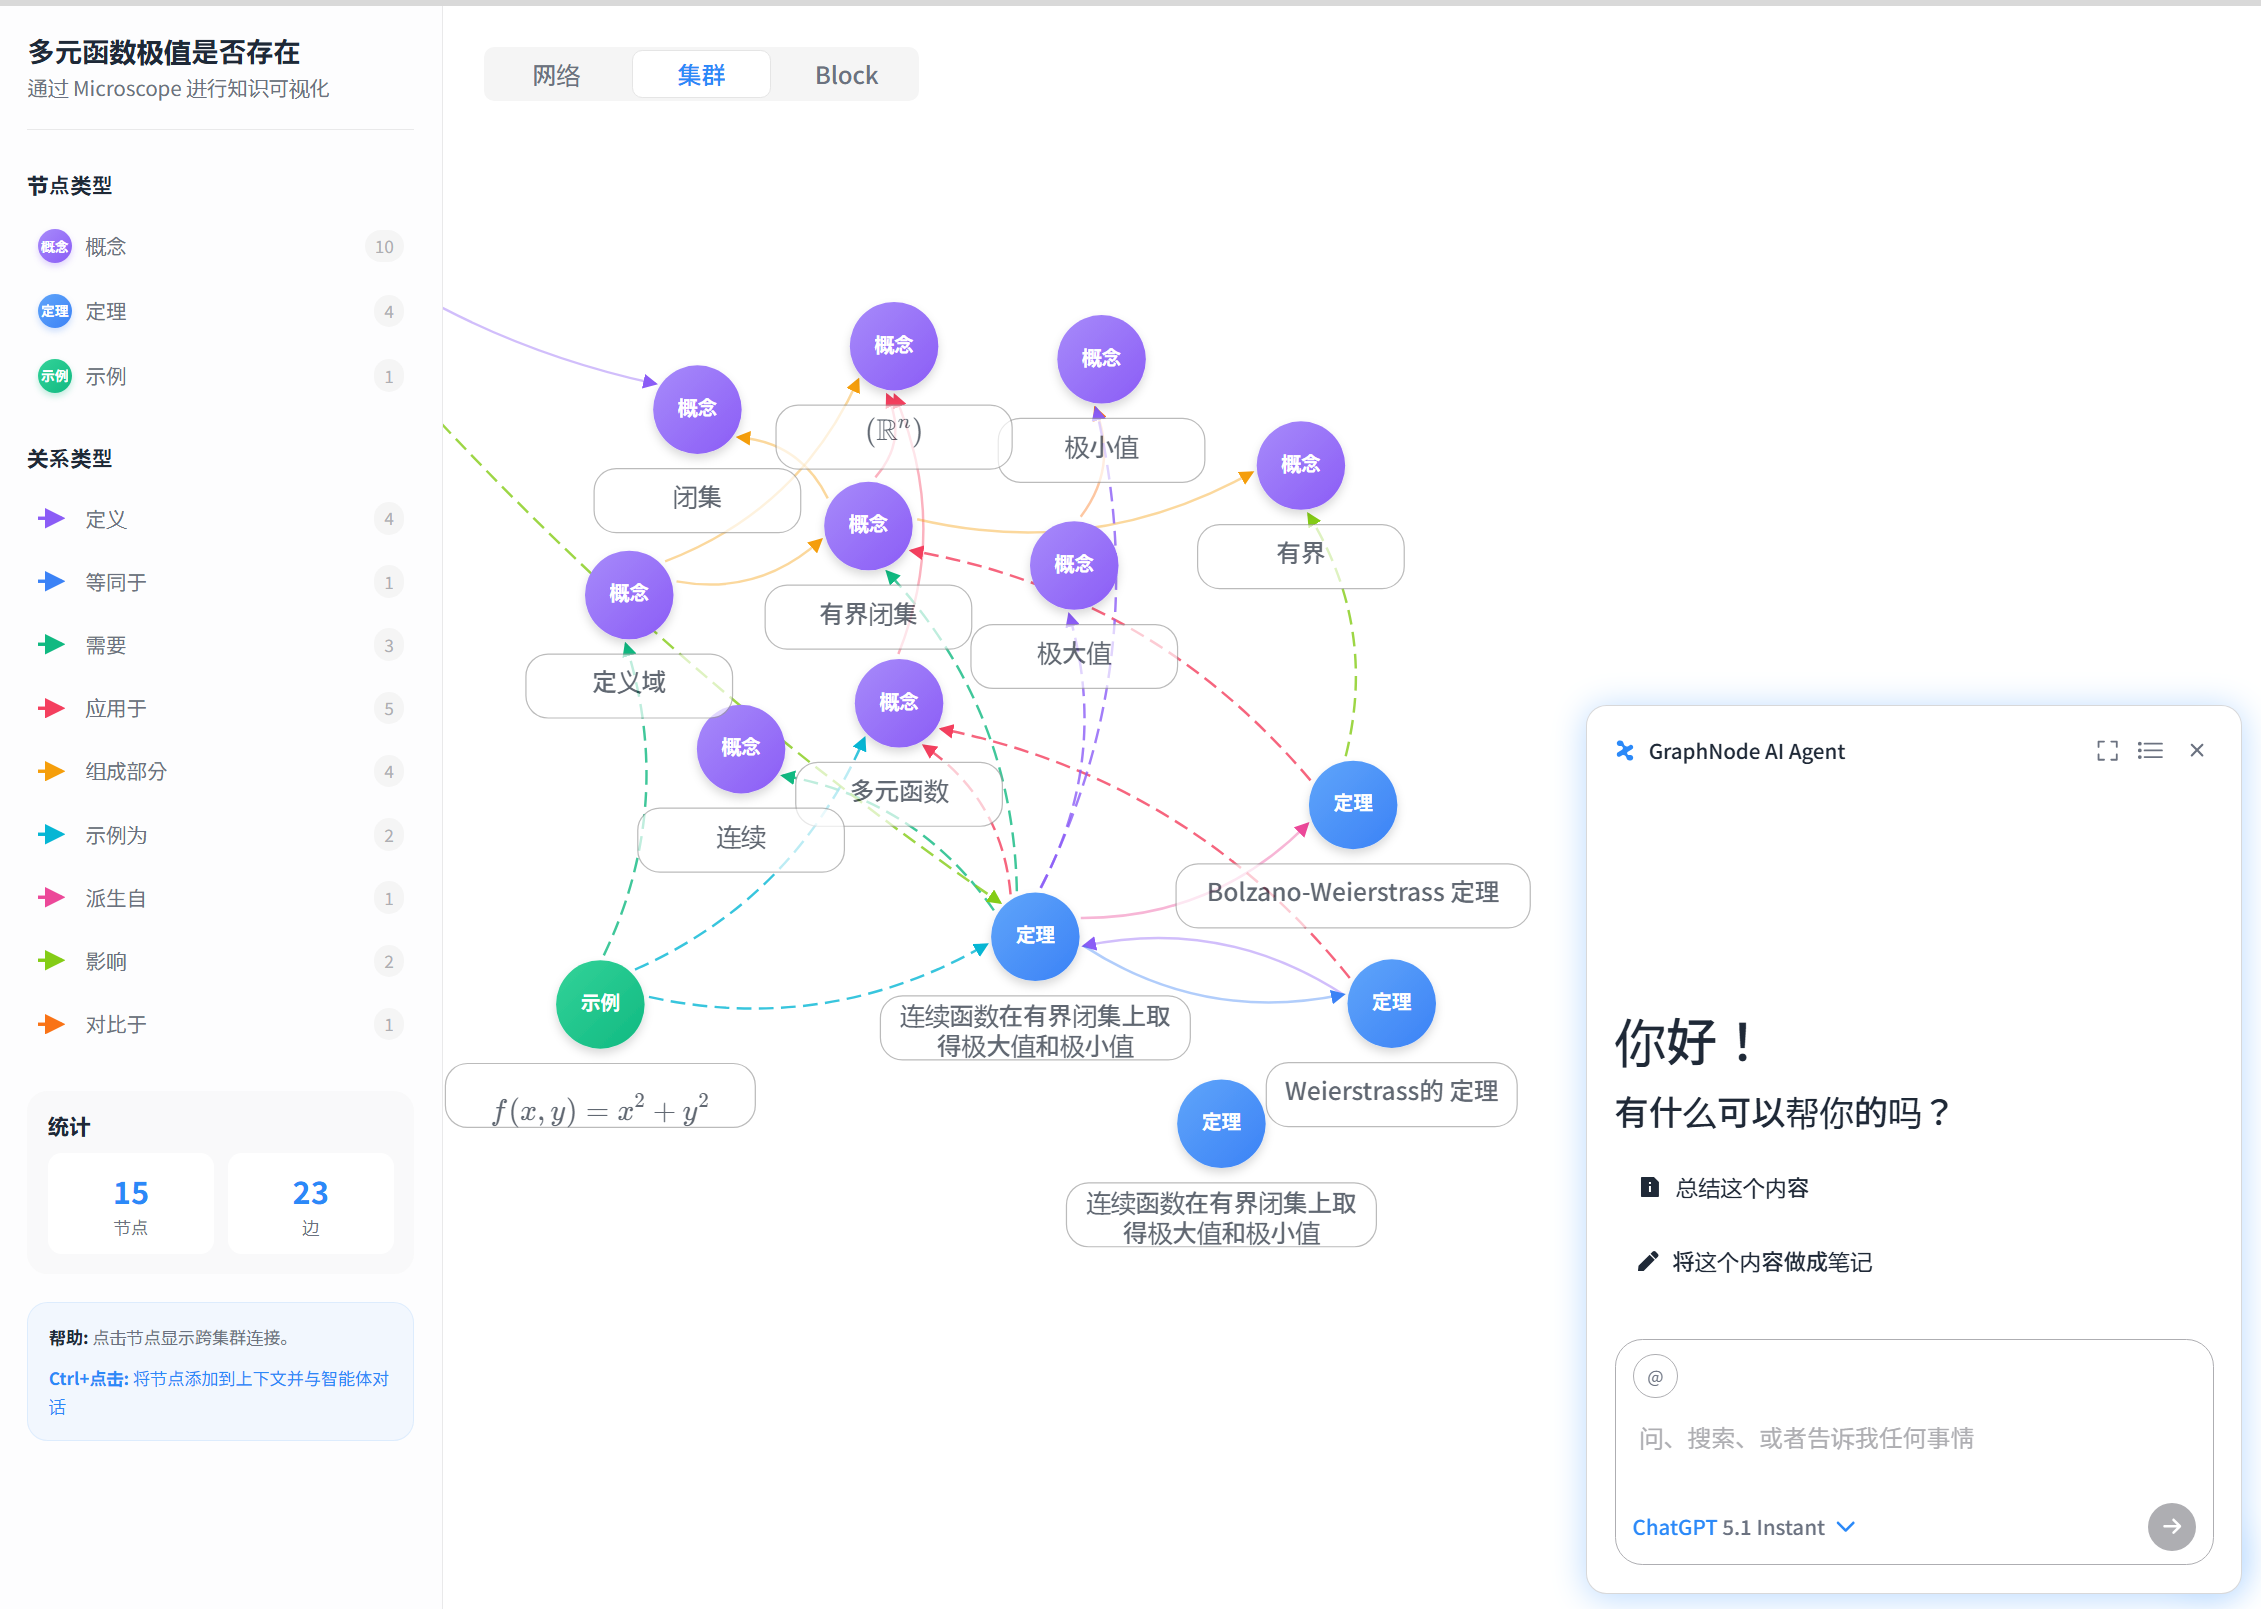
\includegraphics[width=\linewidth, height=15cm, keepaspectratio]{micro_cluster_view.png}\\[-0.1cm]
{\fontsize{22pt}{28pt}\selectfont Cluster View（概念-关系微观图谱）}
\end{minipage}\hfill
\begin{minipage}[t]{0.495\linewidth}\vspace{0pt}\centering
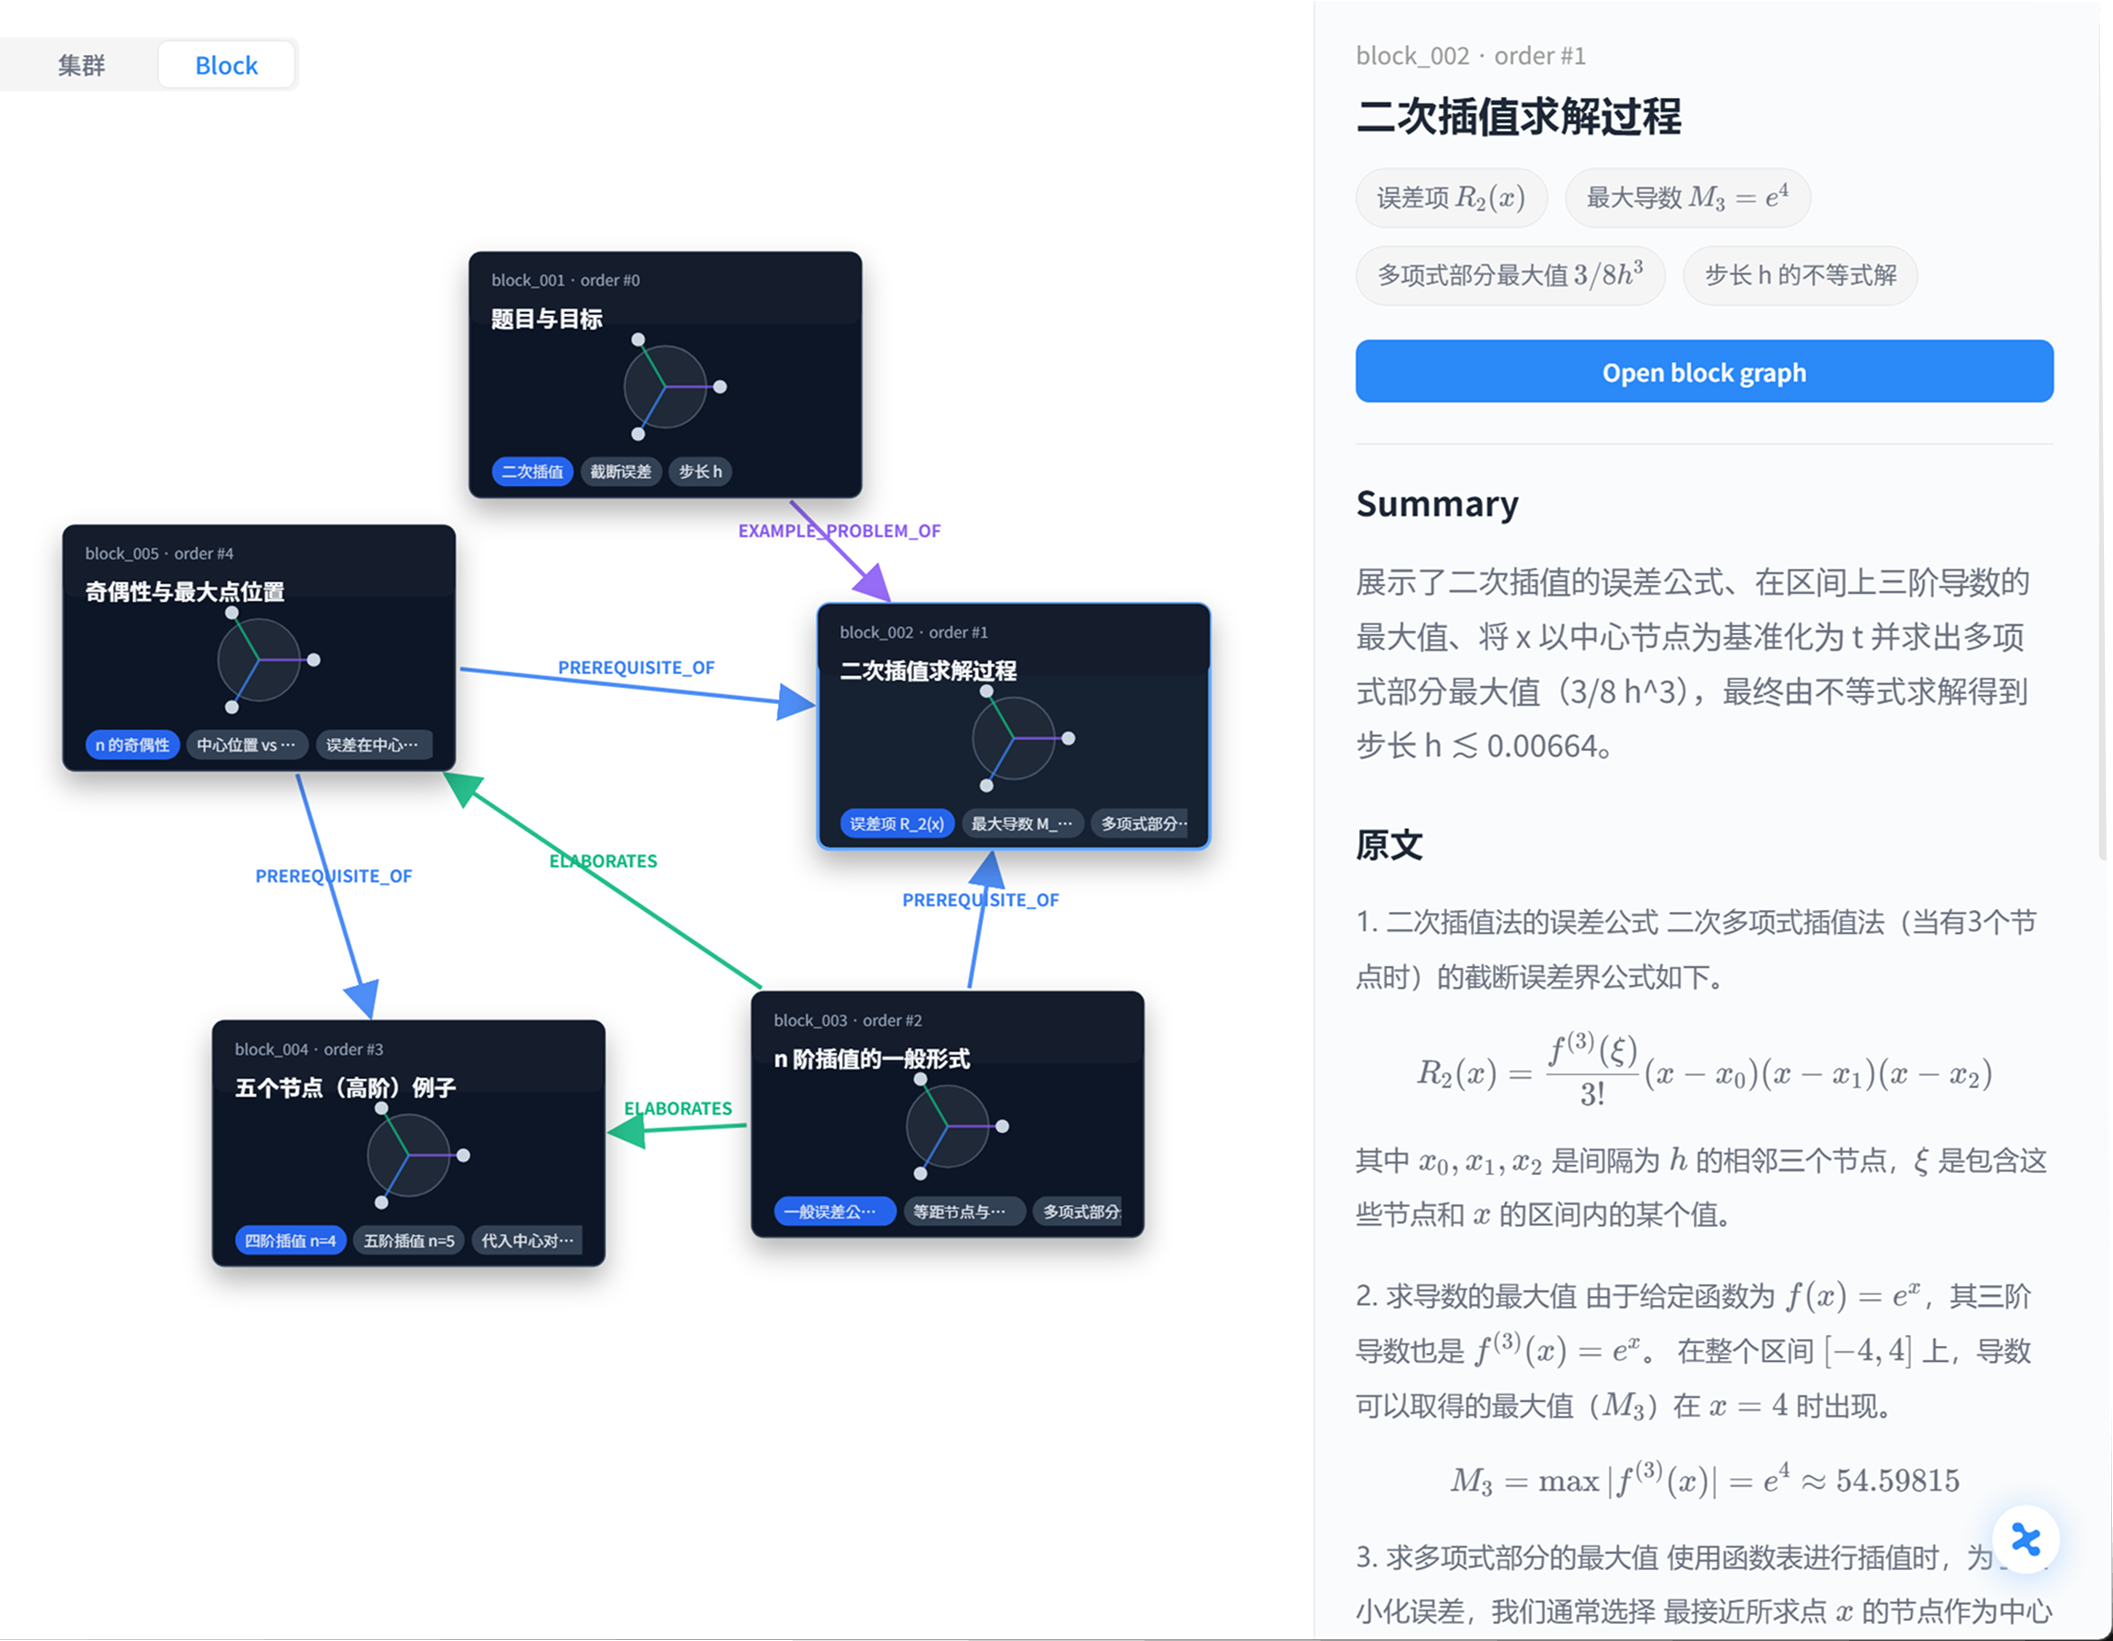
\includegraphics[width=\linewidth, height=15cm, keepaspectratio]{block_view.png}\\[-0.1cm]
{\fontsize{22pt}{28pt}\selectfont Block View（逻辑区块切分）}
\end{minipage}
\end{block}

% ---- 3. Agent Chat (구 4) ----
\begin{block}{3. Agent Chat}
\raggedright
\textbf{交互式问答：基于图谱模块的个性化 RAG}
在任意图谱中点击节点即可唤起 Agent。结合 Macro 模式与用户学习倾向，Agent 能提供超越单轮对话的深度语境回答：

\textbf{【场景一：聚焦 Micro 图谱】}
\textbf{Q：} 这个概念在文中的作用及其与其他概念的关联？ |
\textbf{A（深度解析）：} 基于 Micro 概念网络，梳理上下游逻辑依赖与推导脉络，帮助快速吃透单篇文档结构。

\textbf{【场景二：放眼 Macro 图谱】}
\textbf{Q：} 这个节点与我既有的知识库、其他主题有何联系？ |
\textbf{A（跨域桥接）：} 融合聚类分析，跨越时间与主题定位知识坐标，揭示跨领域的连接关系，帮您俯瞰全局知识版图。\par\medskip
\noindent
\begin{minipage}[t]{0.495\linewidth}\vspace{0pt}\centering
\begin{minipage}[t][13.5cm][t]{\linewidth}\centering
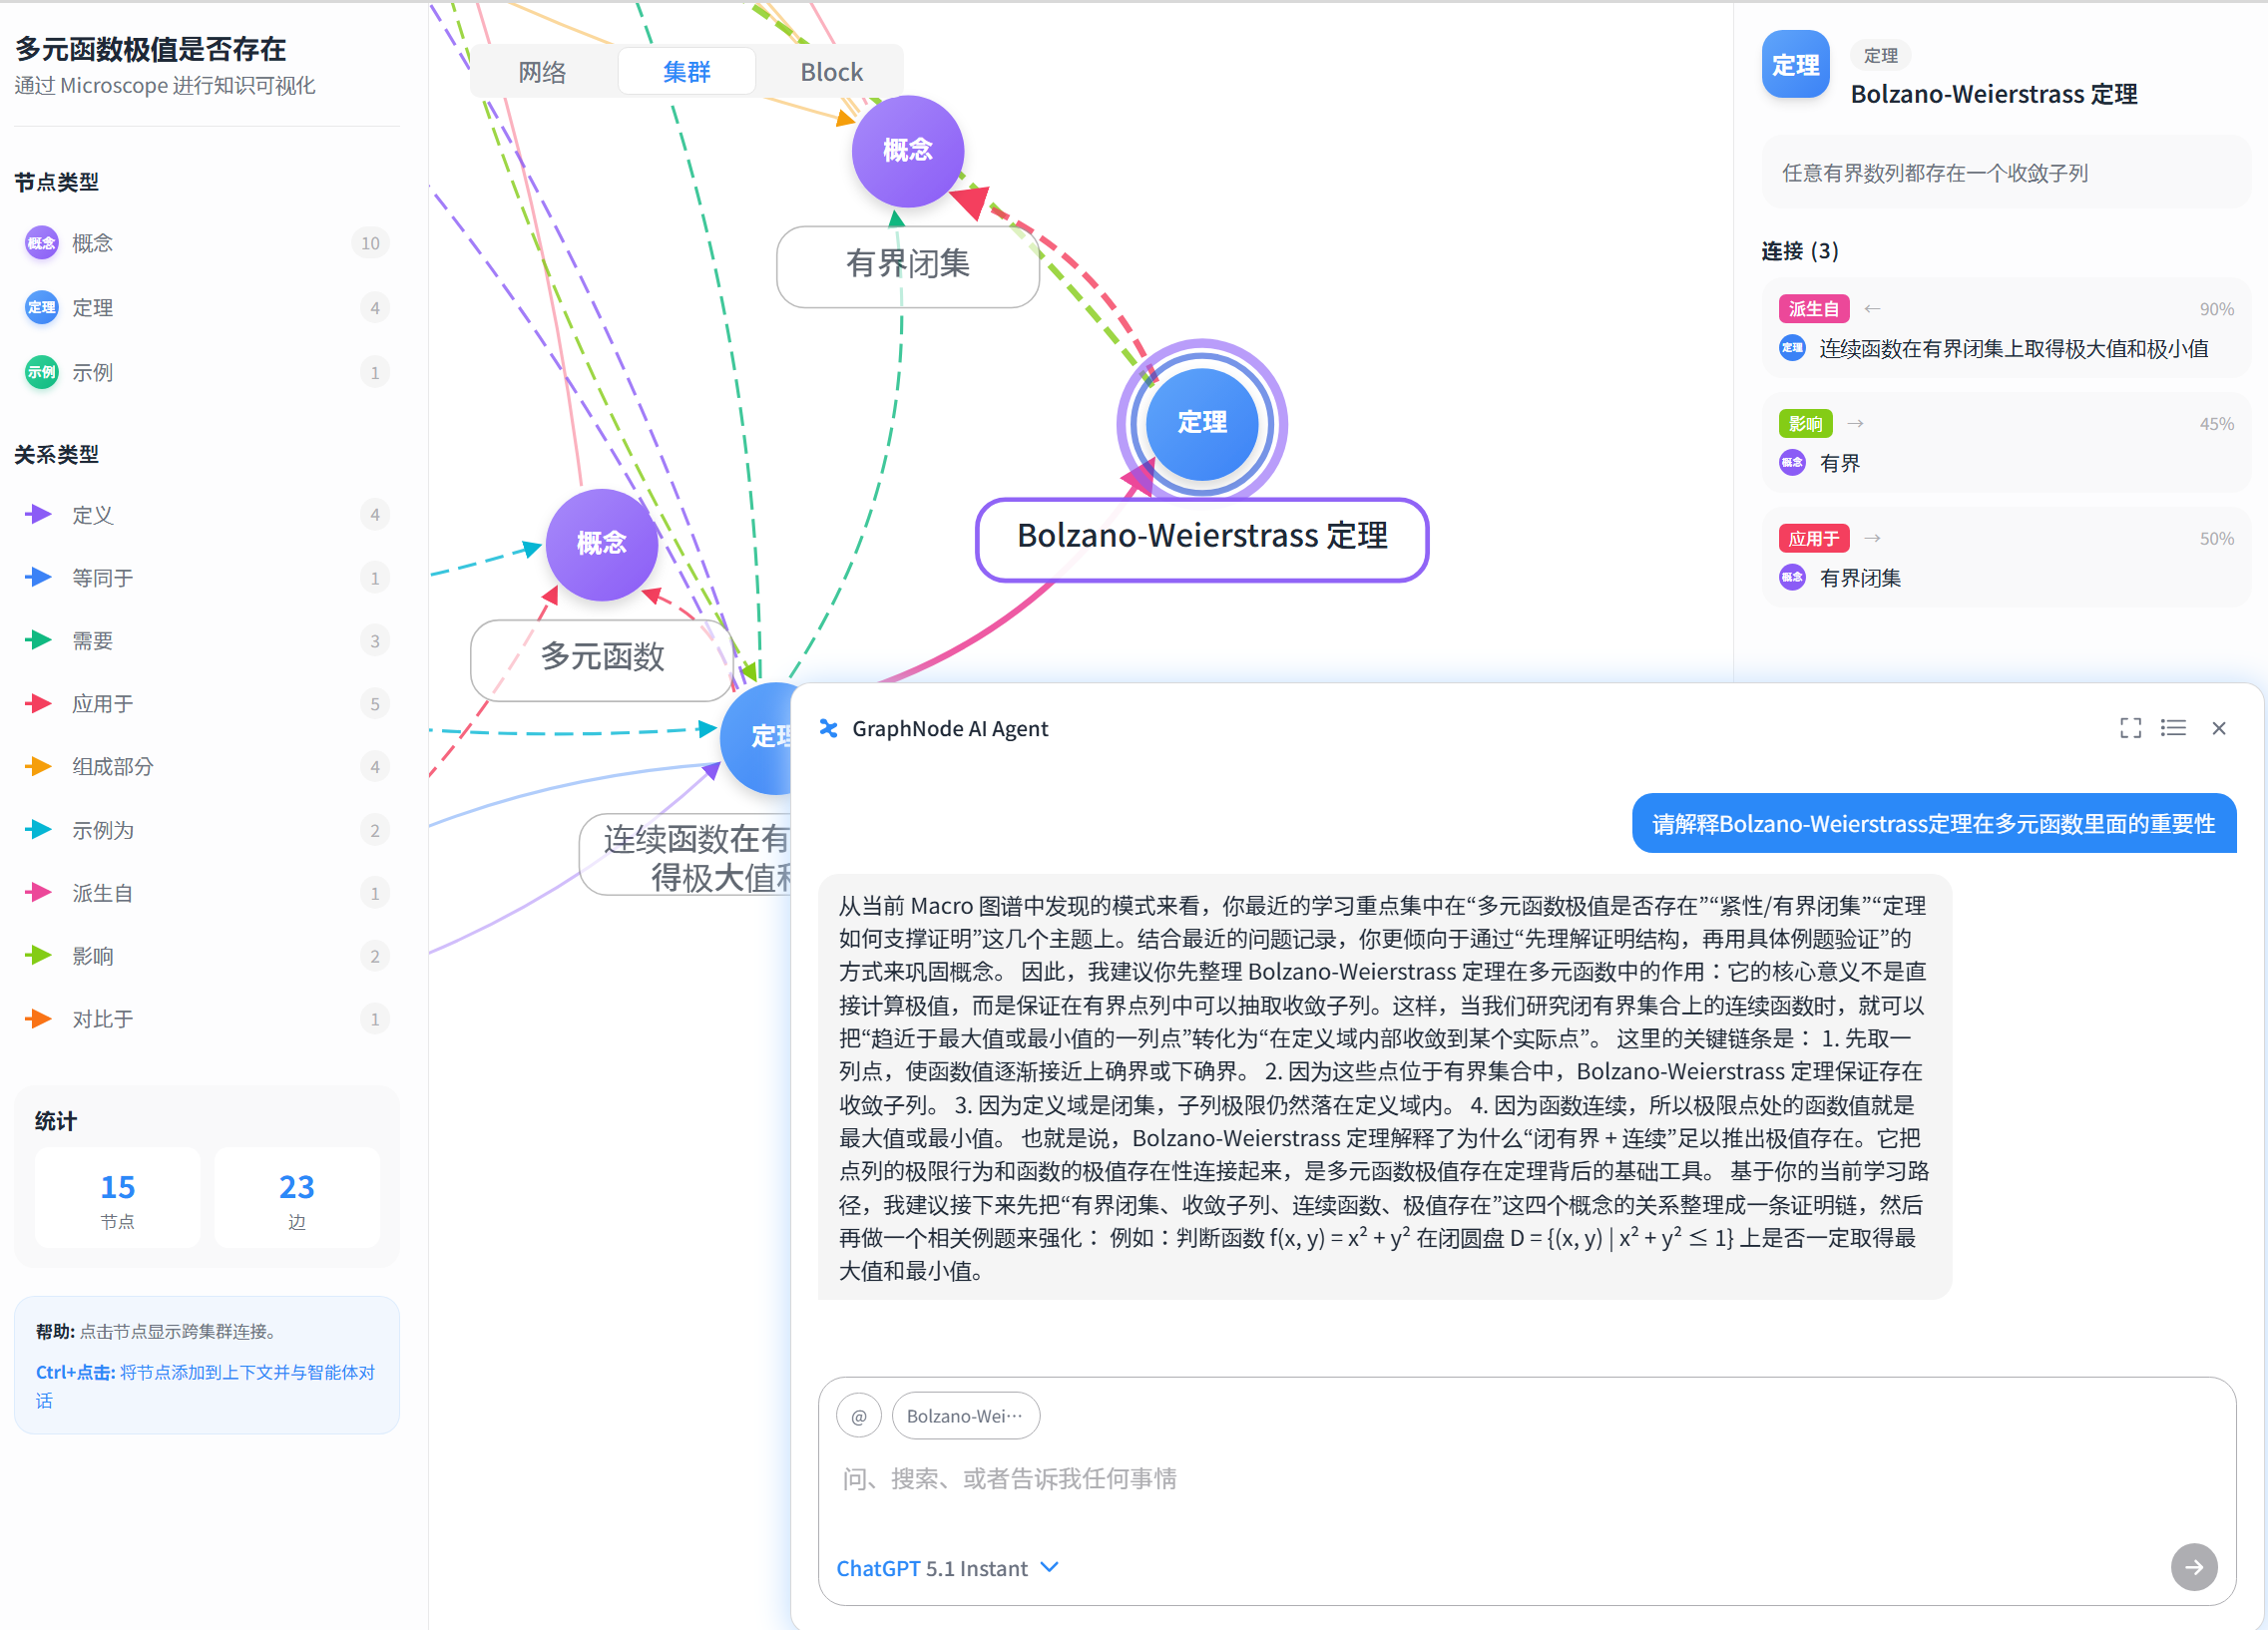
\includegraphics[width=\linewidth, height=13.5cm, keepaspectratio]{cluster_view_agent.png}
\end{minipage}\\[-0.1cm]
{\fontsize{22pt}{28pt}\selectfont Micro 节点 → 单篇语境深挖}
\end{minipage}\hfill
\begin{minipage}[t]{0.495\linewidth}\vspace{0pt}\centering
\begin{minipage}[t][13.5cm][t]{\linewidth}\centering
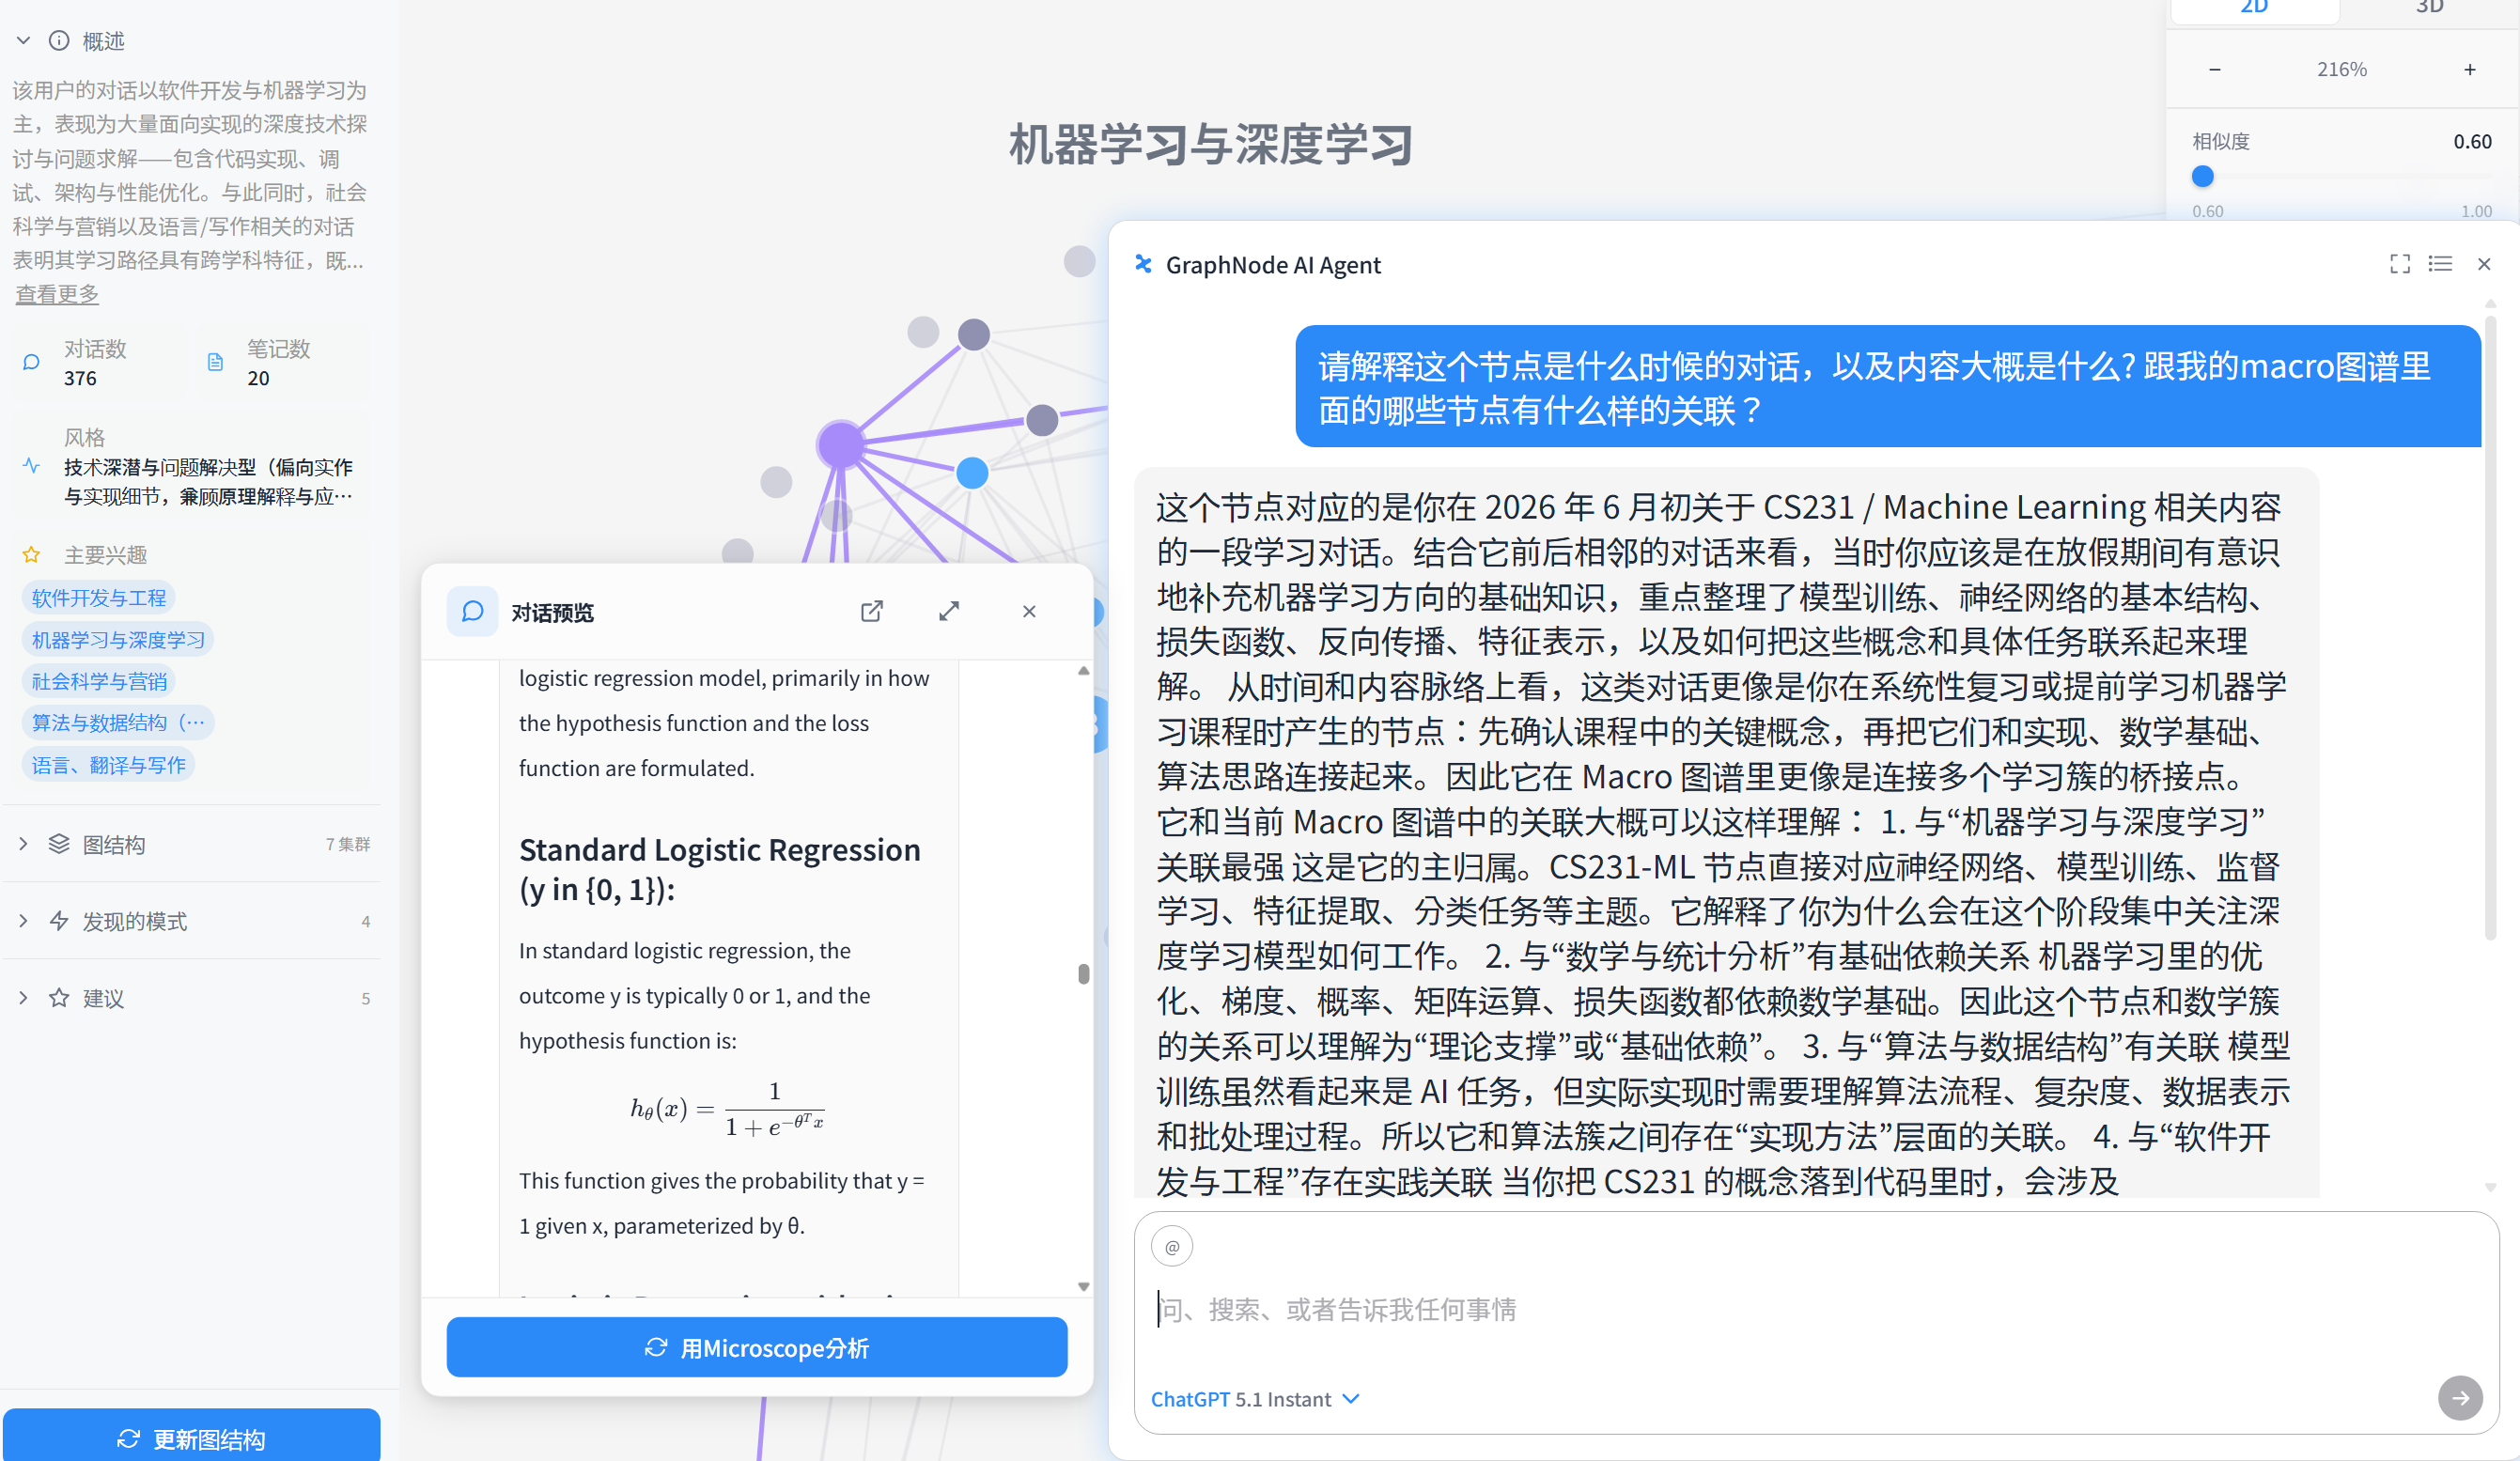
\includegraphics[width=\linewidth, height=13.5cm, keepaspectratio]{macro_agent.png}
\end{minipage}\\[-0.1cm]
{\fontsize{22pt}{28pt}\selectfont Macro 节点 → 俯瞰全局关联}
\end{minipage}
\end{block}

\end{column}

%========================== 오른쪽 단 ==========================
\begin{column}{0.46\paperwidth}
\fontsize{36pt}{46pt}\selectfont

% % ---- 4. 数据输入 & 笔记编辑器 (구 2) ----
% \begin{block}{4. 数据输入 \& 笔记编辑器}
% 此模块是 Macro / Micro 图谱的源头（Source）：所有对话与笔记都将作为知识图谱生成的原始素材。
% \raggedright
% \textbf{数据输入}：内置 AI 对话（ChatGPT / Claude / Gemini），并支持\textbf{外部数据导入 / 导出}
% （Json / ZIP / Markdown）。\\[0.2cm]
% \textbf{笔记编辑器}：提供媲美 \textbf{Notion / Obsidian} 的流畅编辑体验（支持 Markdown 语法、高亮、html等），并支持 \textbf{docx / PDF / pptx} 等多种格式文档的查看与解析。
% \vspace{-0.1cm}\\
% \noindent
% \begin{minipage}[t]{0.495\linewidth}\vspace{0pt}\centering
% 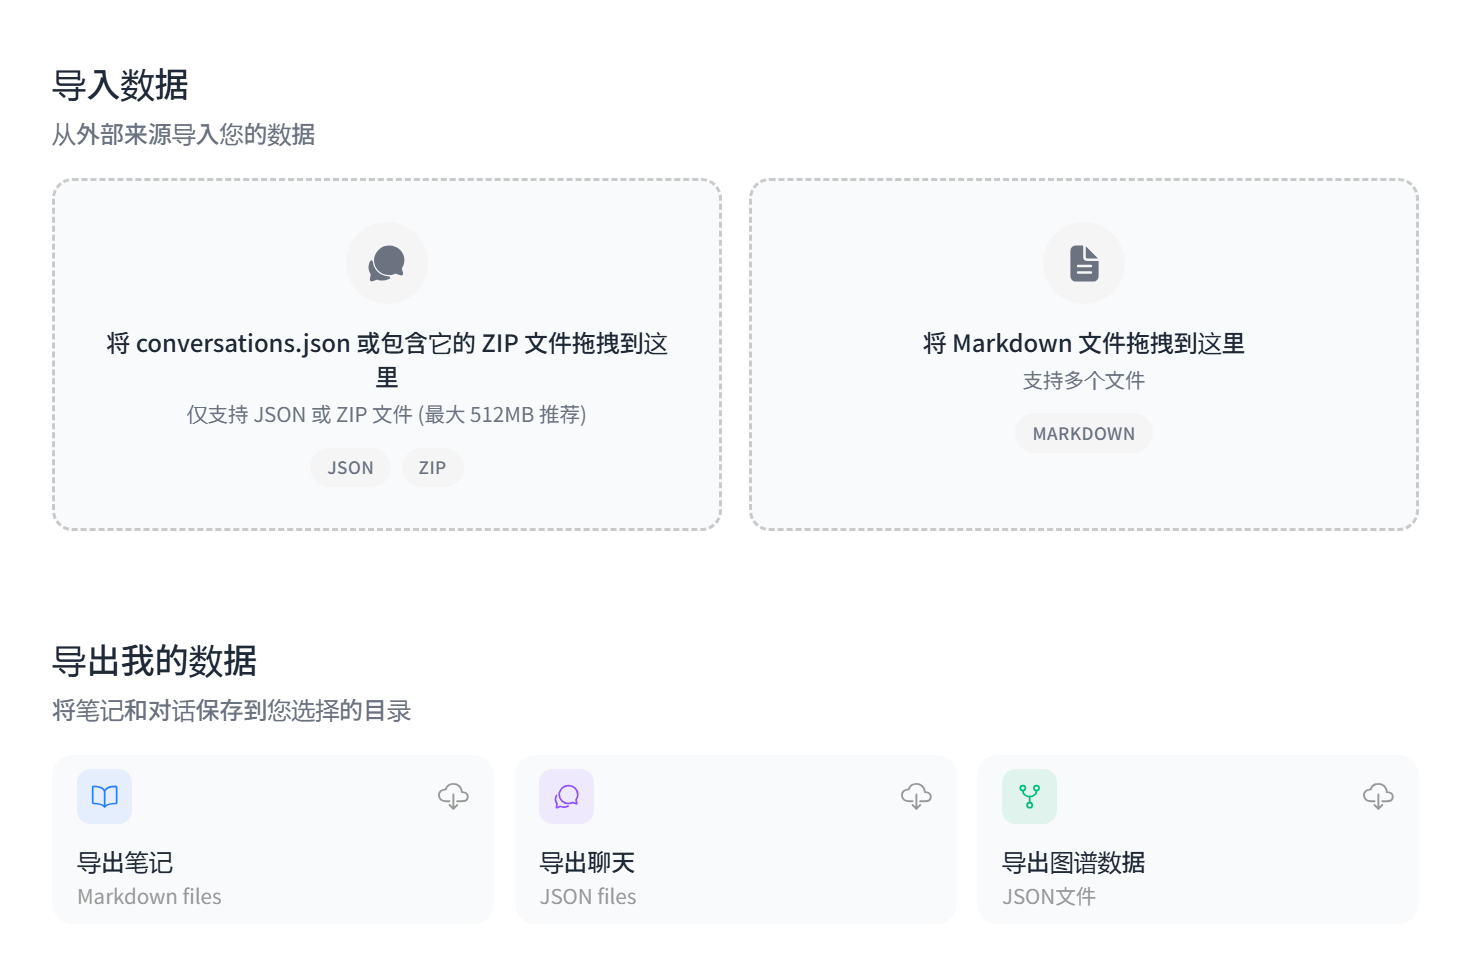
\includegraphics[width=\linewidth, height=12cm, keepaspectratio]{import_export_data.png}\\[-0.1cm]
% {\fontsize{22pt}{28pt}\selectfont 数据导入/导出}
% \end{minipage}\hfill
% \begin{minipage}[t]{0.495\linewidth}\vspace{0pt}\centering
% 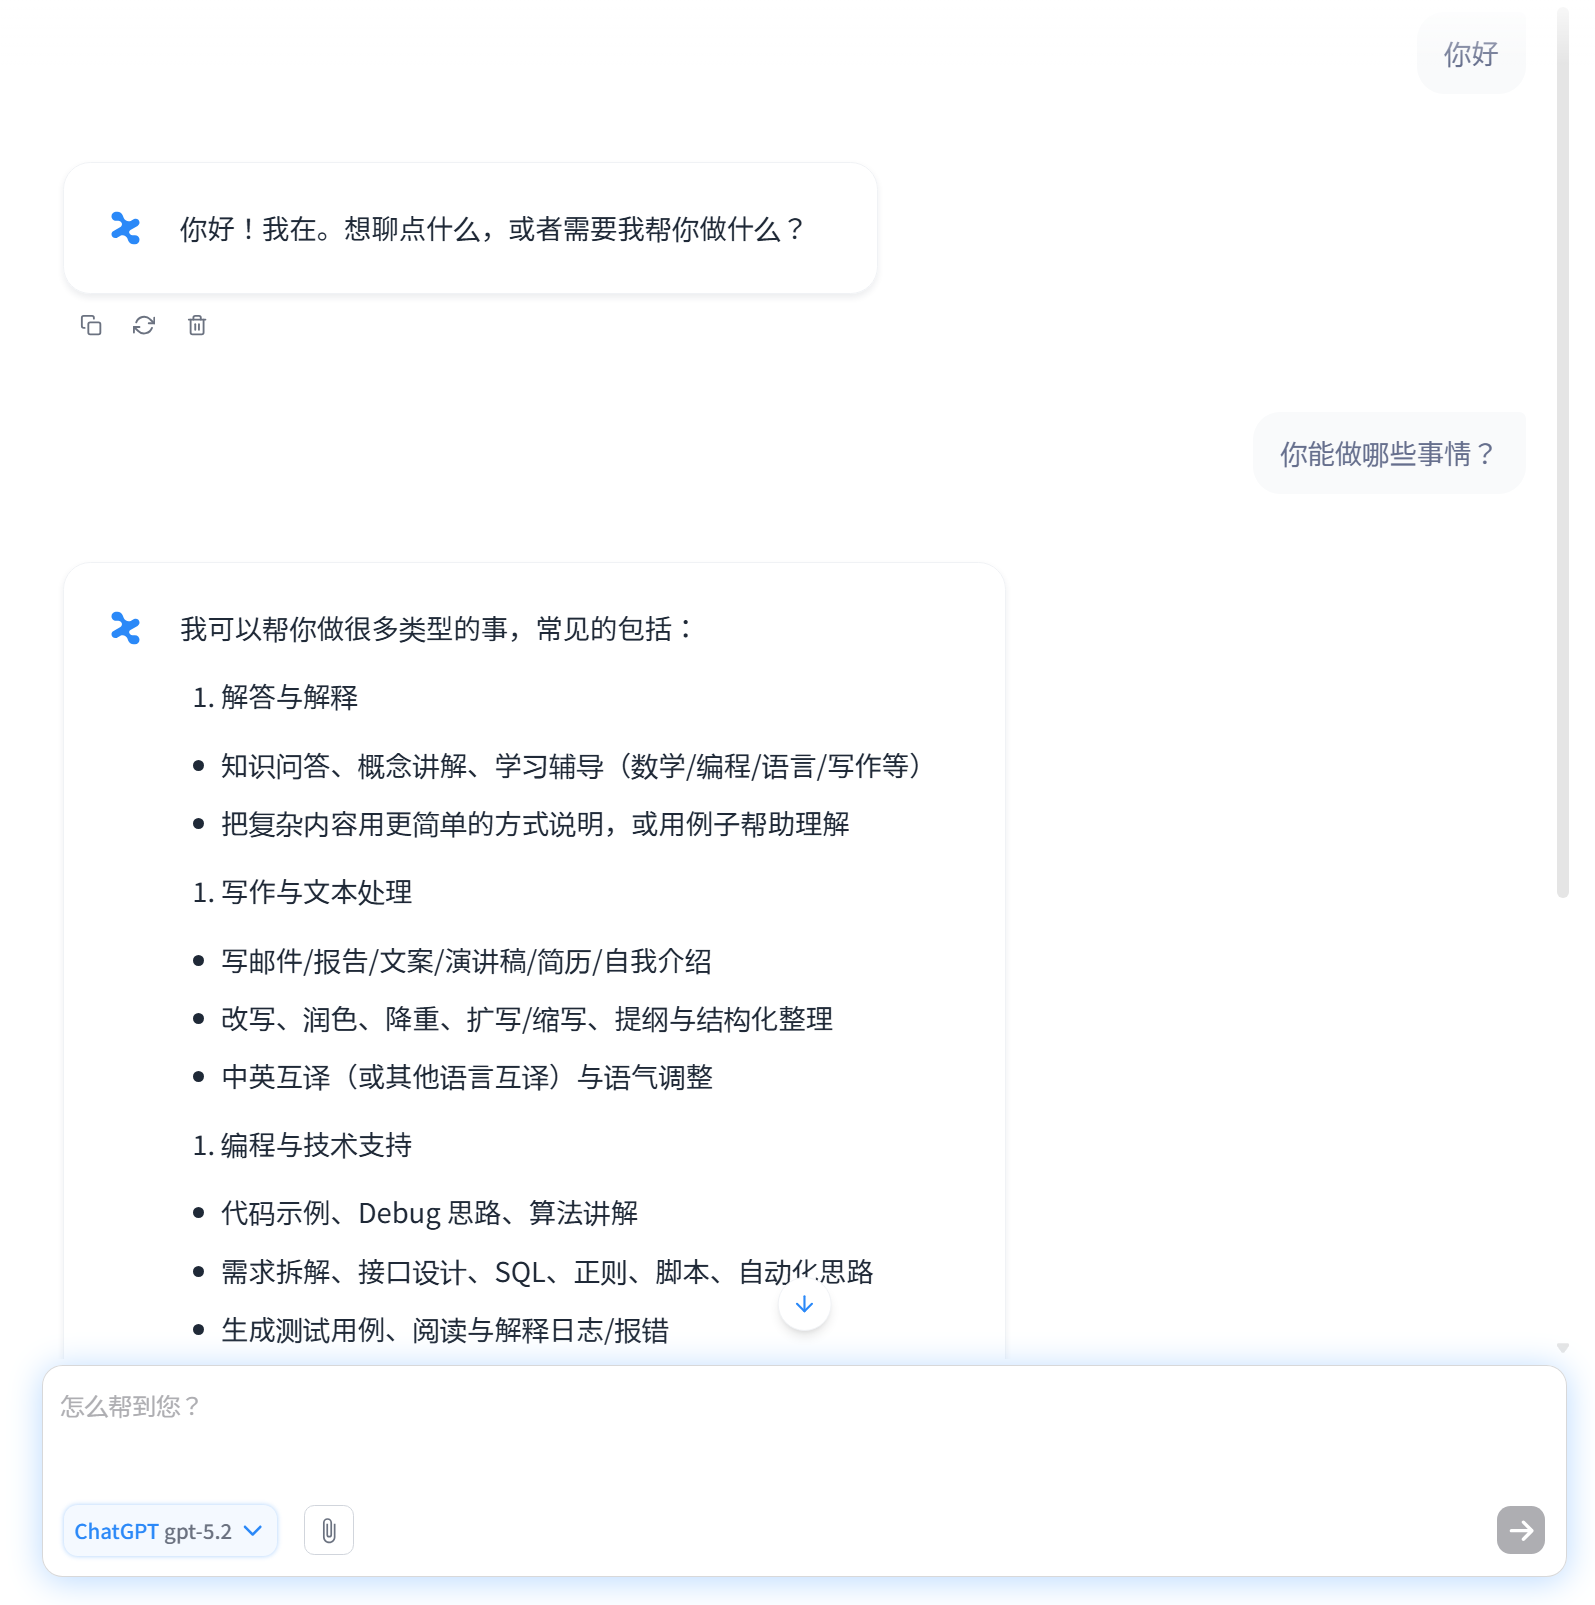
\includegraphics[width=\linewidth, height=12cm, keepaspectratio]{ai_conversation.png}\\[-0.1cm]
% {\fontsize{22pt}{28pt}\selectfont 内置AI对话}
% \end{minipage}\\[0cm]
% \noindent
% \begin{minipage}[t]{0.495\linewidth}\vspace{0pt}\centering
% 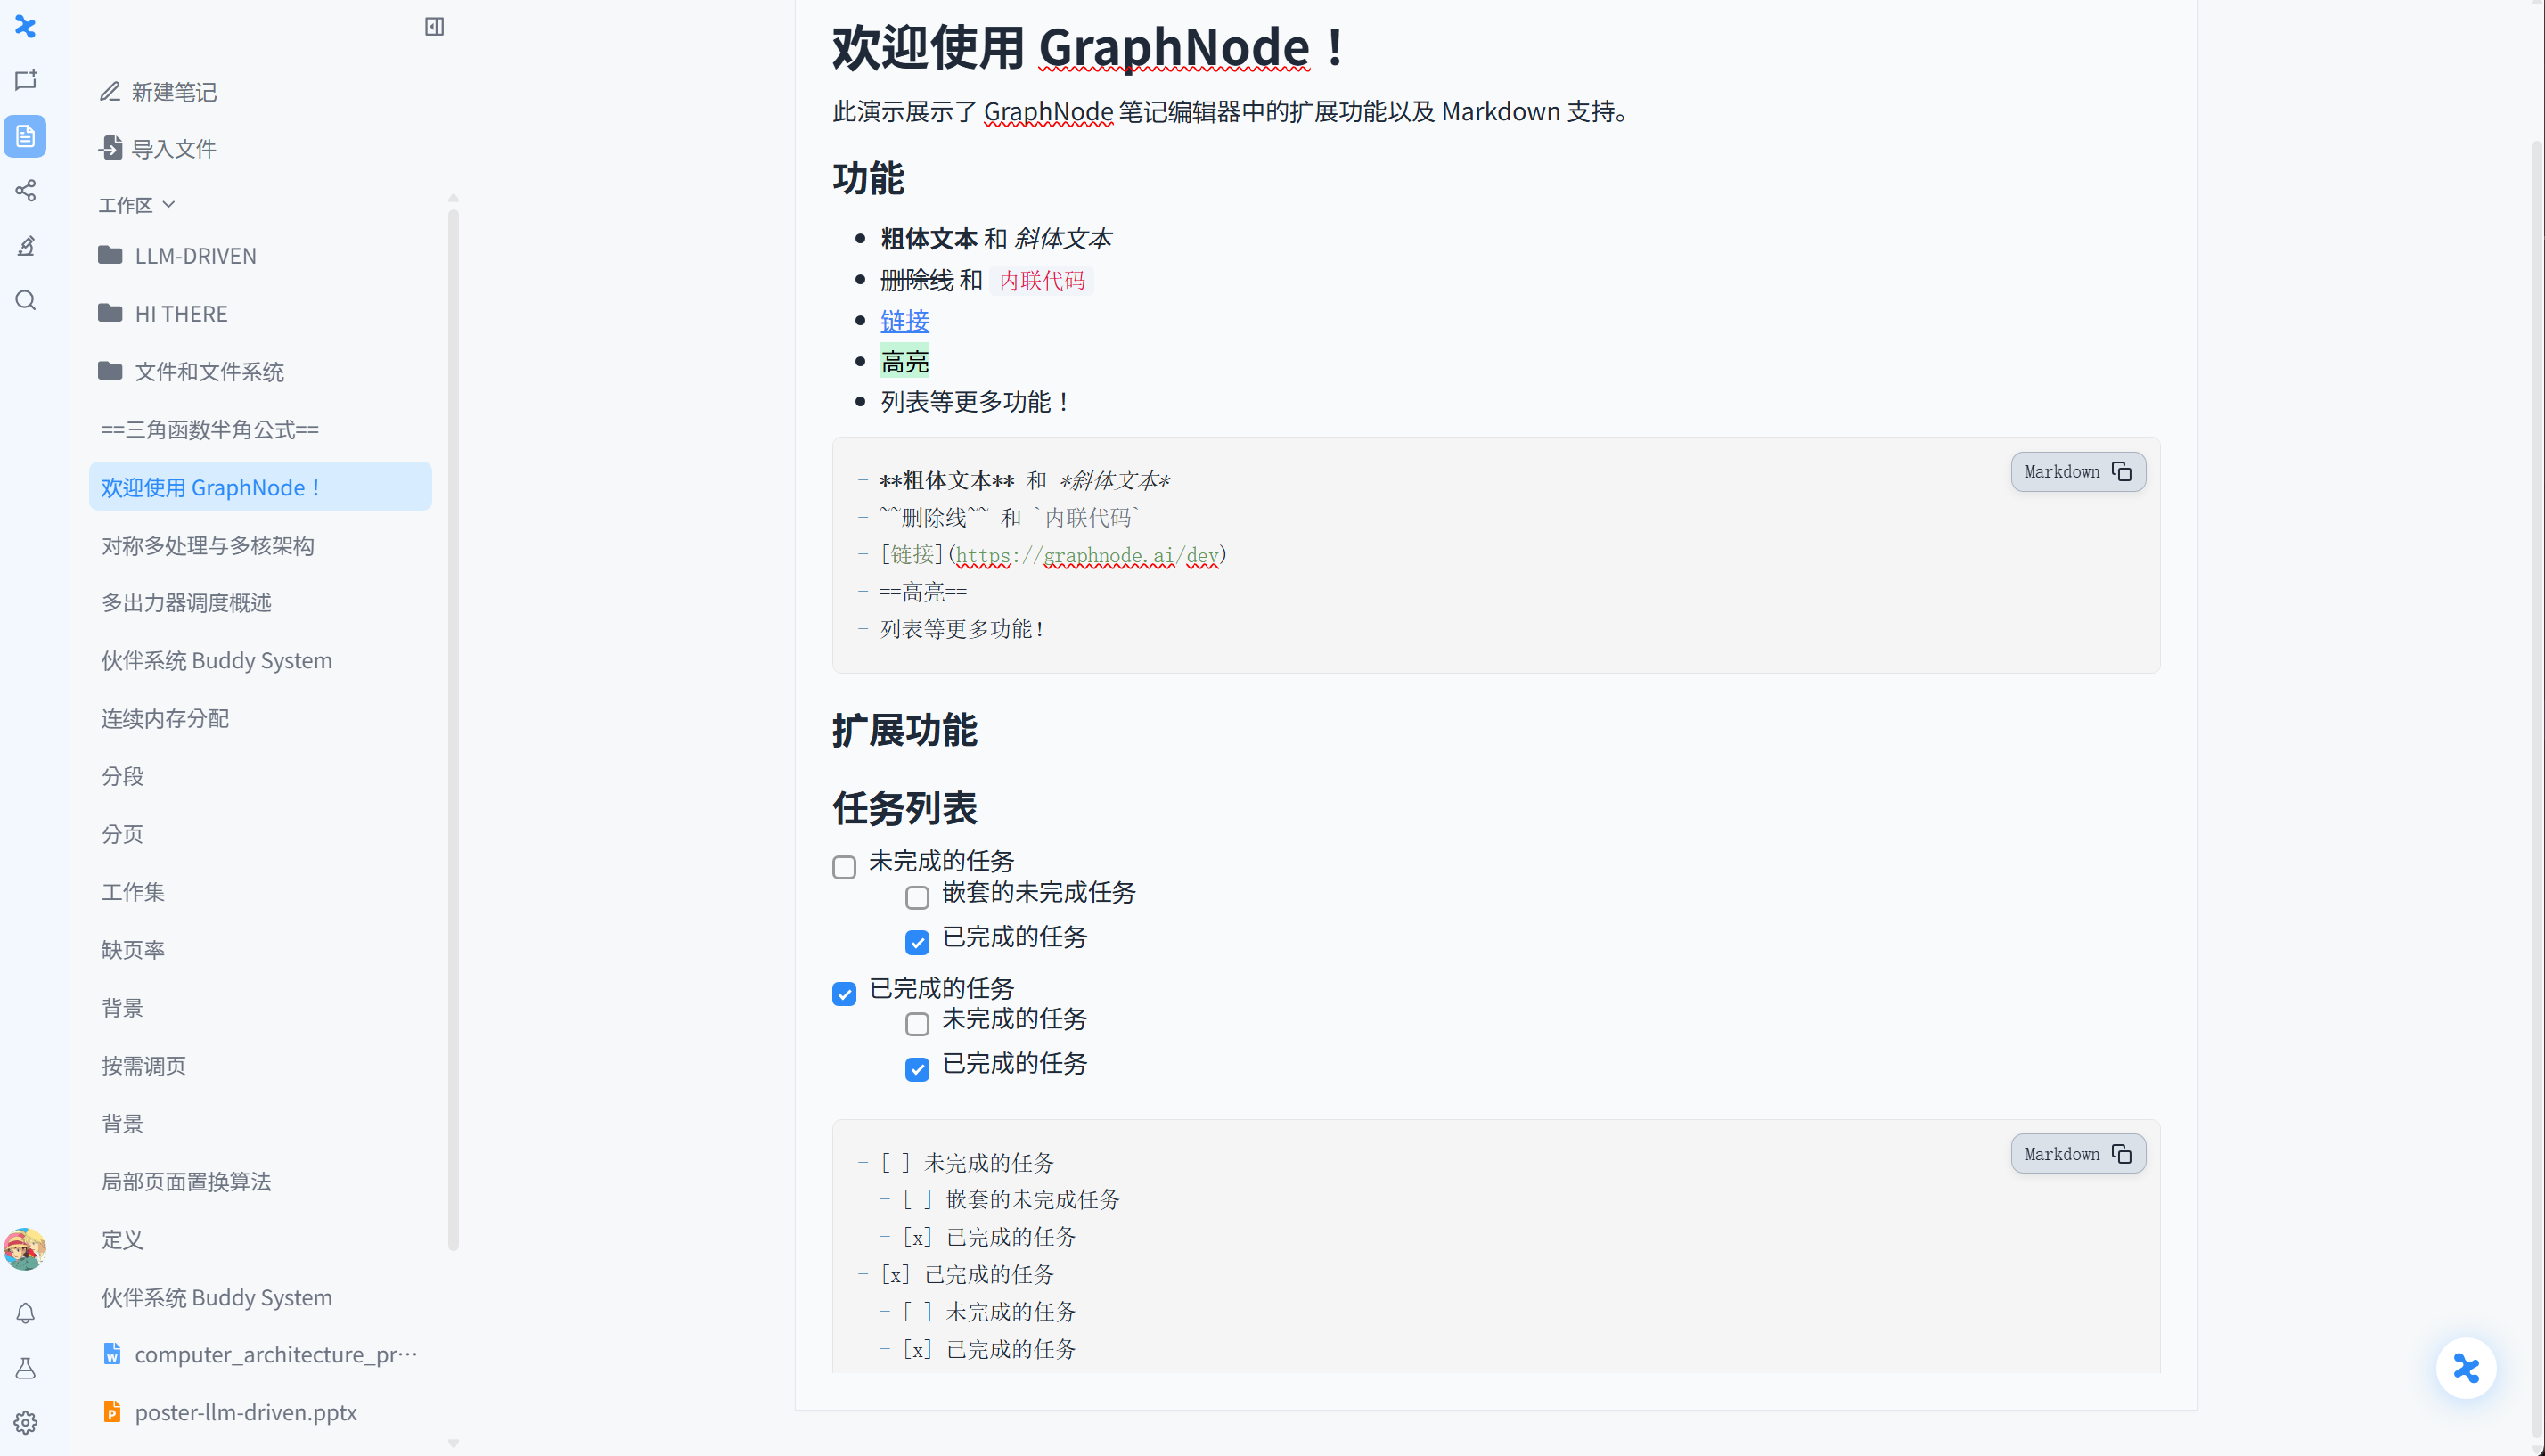
\includegraphics[width=\linewidth, height=12cm, keepaspectratio]{graphnode_note.png}\\[-0.1cm]
% {\fontsize{22pt}{28pt}\selectfont 笔记编辑器}
% \end{minipage}\hfill
% \begin{minipage}[t]{0.495\linewidth}\vspace{0pt}\centering
% 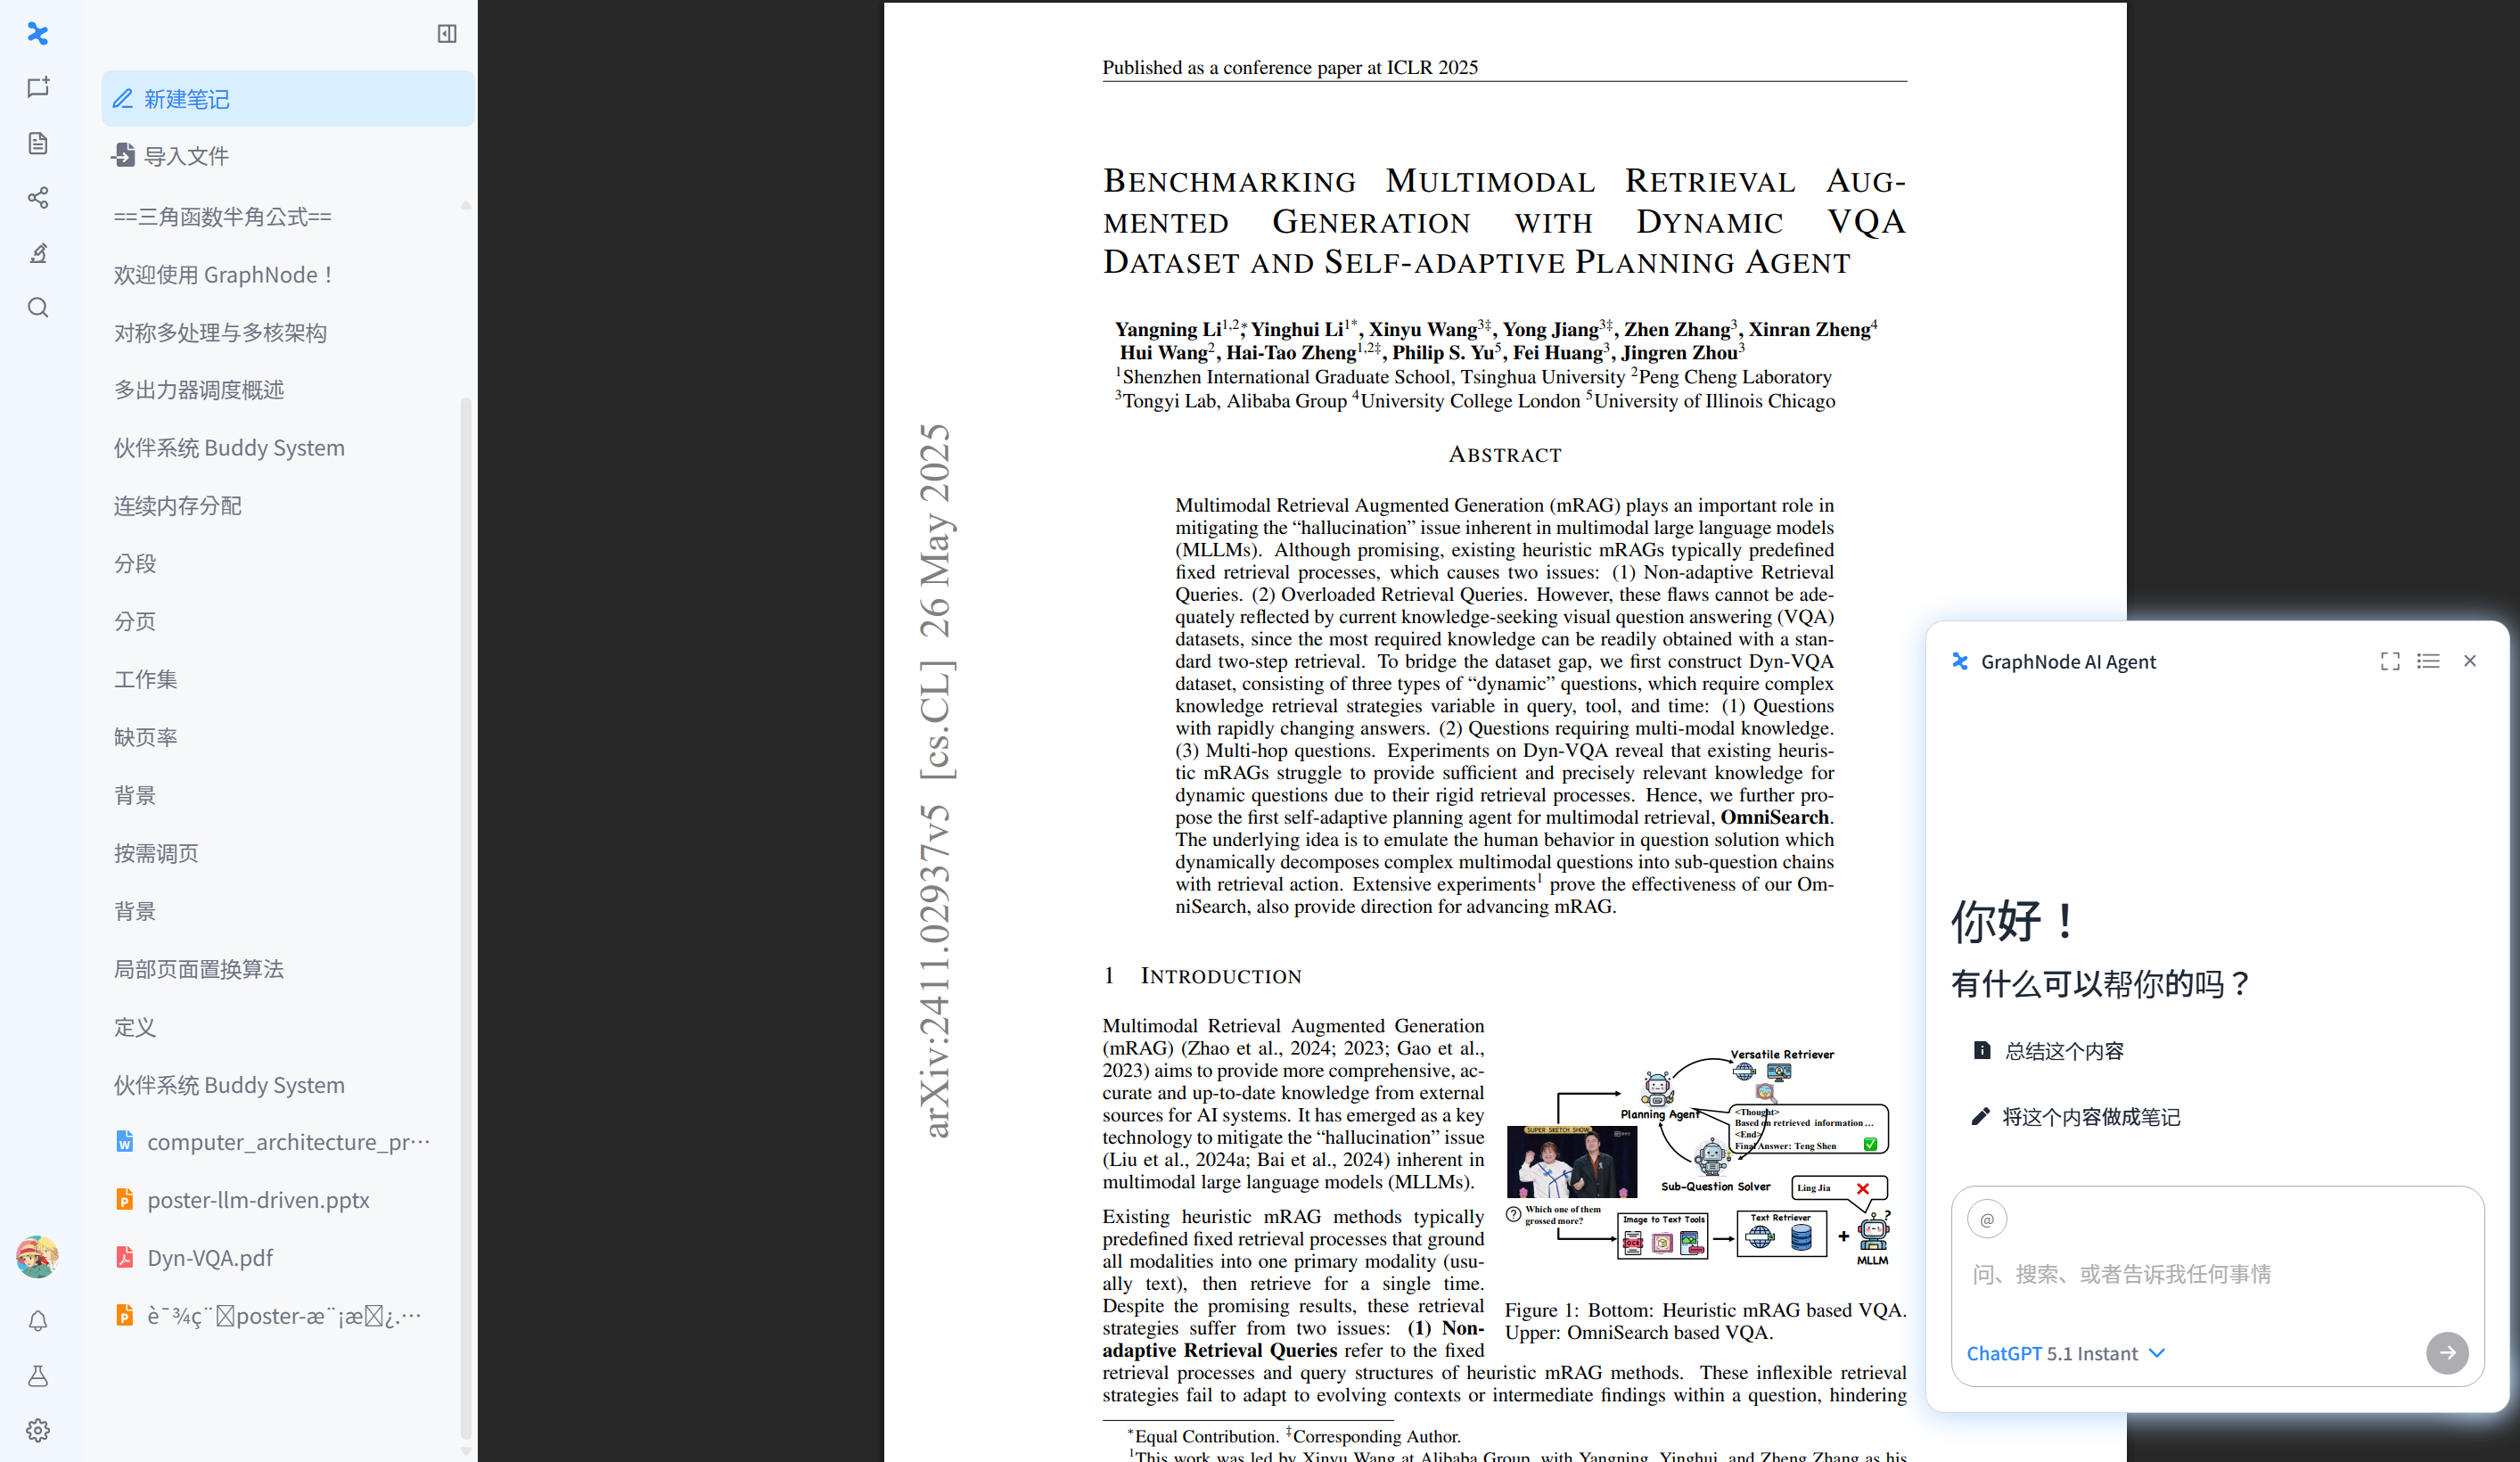
\includegraphics[width=\linewidth, height=12cm, keepaspectratio]{pdf_viewr_with_agent.png}\\[-0.1cm]
% {\fontsize{22pt}{28pt}\selectfont PDF 查看}
% \end{minipage}
% \end{block}
% ---- 4. 知识采集与沉淀：图谱生成的源数据层 ----
\begin{block}{4. 知识采集：图谱生成的源数据层}
\raggedright
\textbf{数据导入与内置AI对话}：内置 AI 对话（ChatGPT / Claude / Gemini）并支持跨平台数据导入（JSON / ZIP / Markdown），将散落在各处的对话转化为构建 Macro / Micro 图谱的\textbf{结构化语义素材}。\\[0.2cm]

\textbf{笔记编辑器}：提供媲美 \textbf{Notion / Obsidian} 的流畅编辑体验，并支持 \textbf{docx / pdf / pptx} 等多种格式文档的查看。在此沉淀的每一条笔记与文献，均是能\textbf{转化为 Macro / Micro 图谱核心节点的直接源数据}。

\vspace{0.3cm}
\noindent
\begin{minipage}[t]{0.495\linewidth}\vspace{0pt}\centering
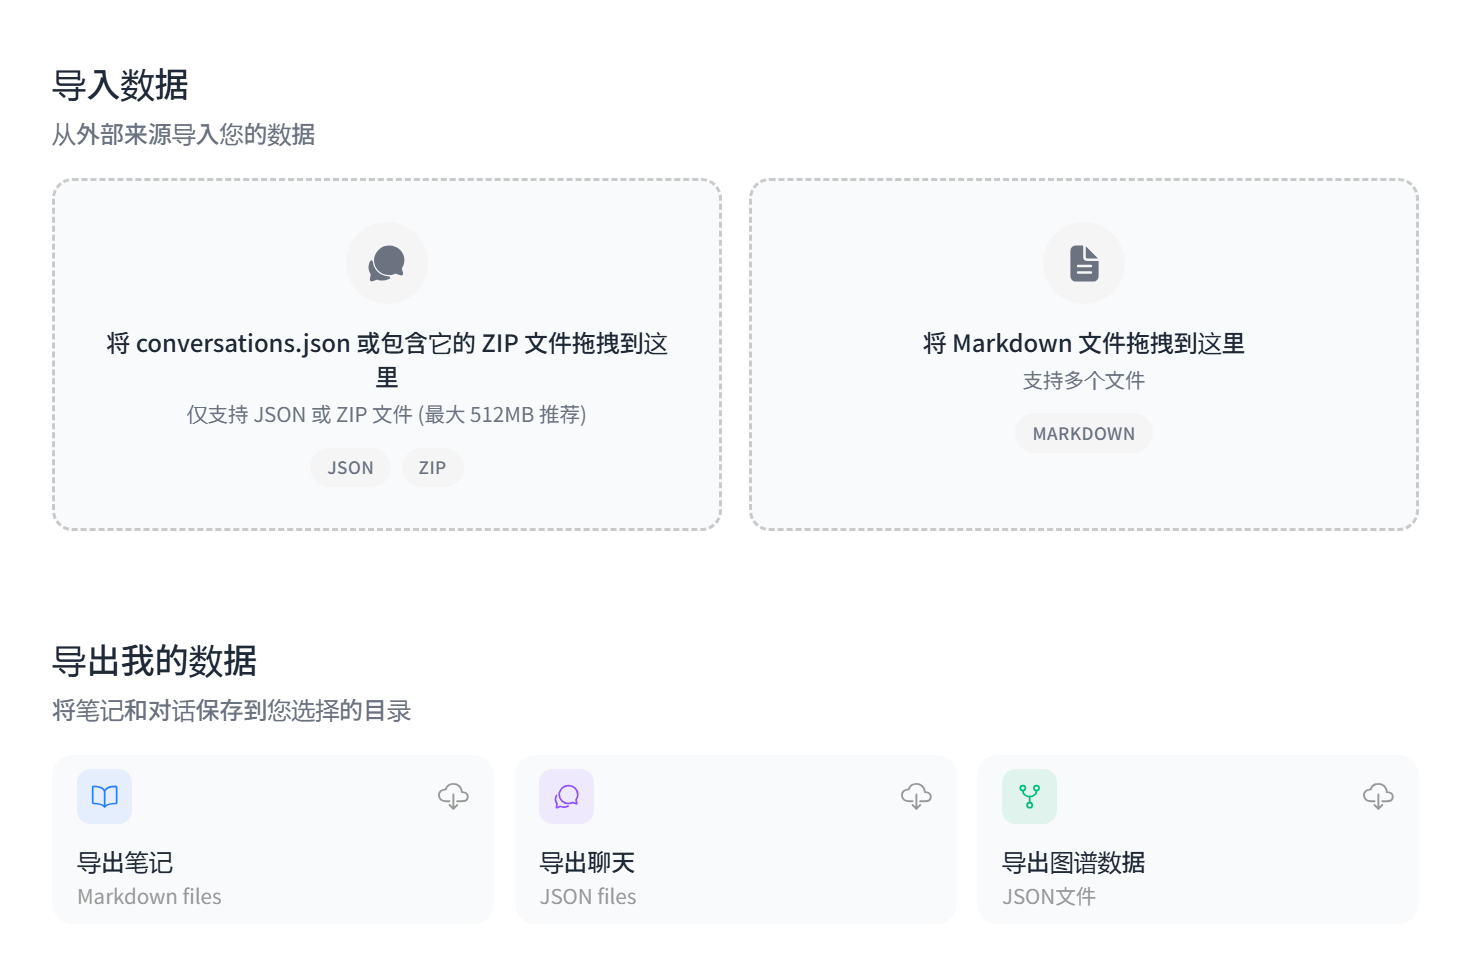
\includegraphics[width=\linewidth, height=12cm, keepaspectratio]{import_export_data.png}\\[-0.1cm]
{\fontsize{22pt}{28pt}\selectfont 多源数据导入/导出}
\end{minipage}\hfill
\begin{minipage}[t]{0.495\linewidth}\vspace{0pt}\centering
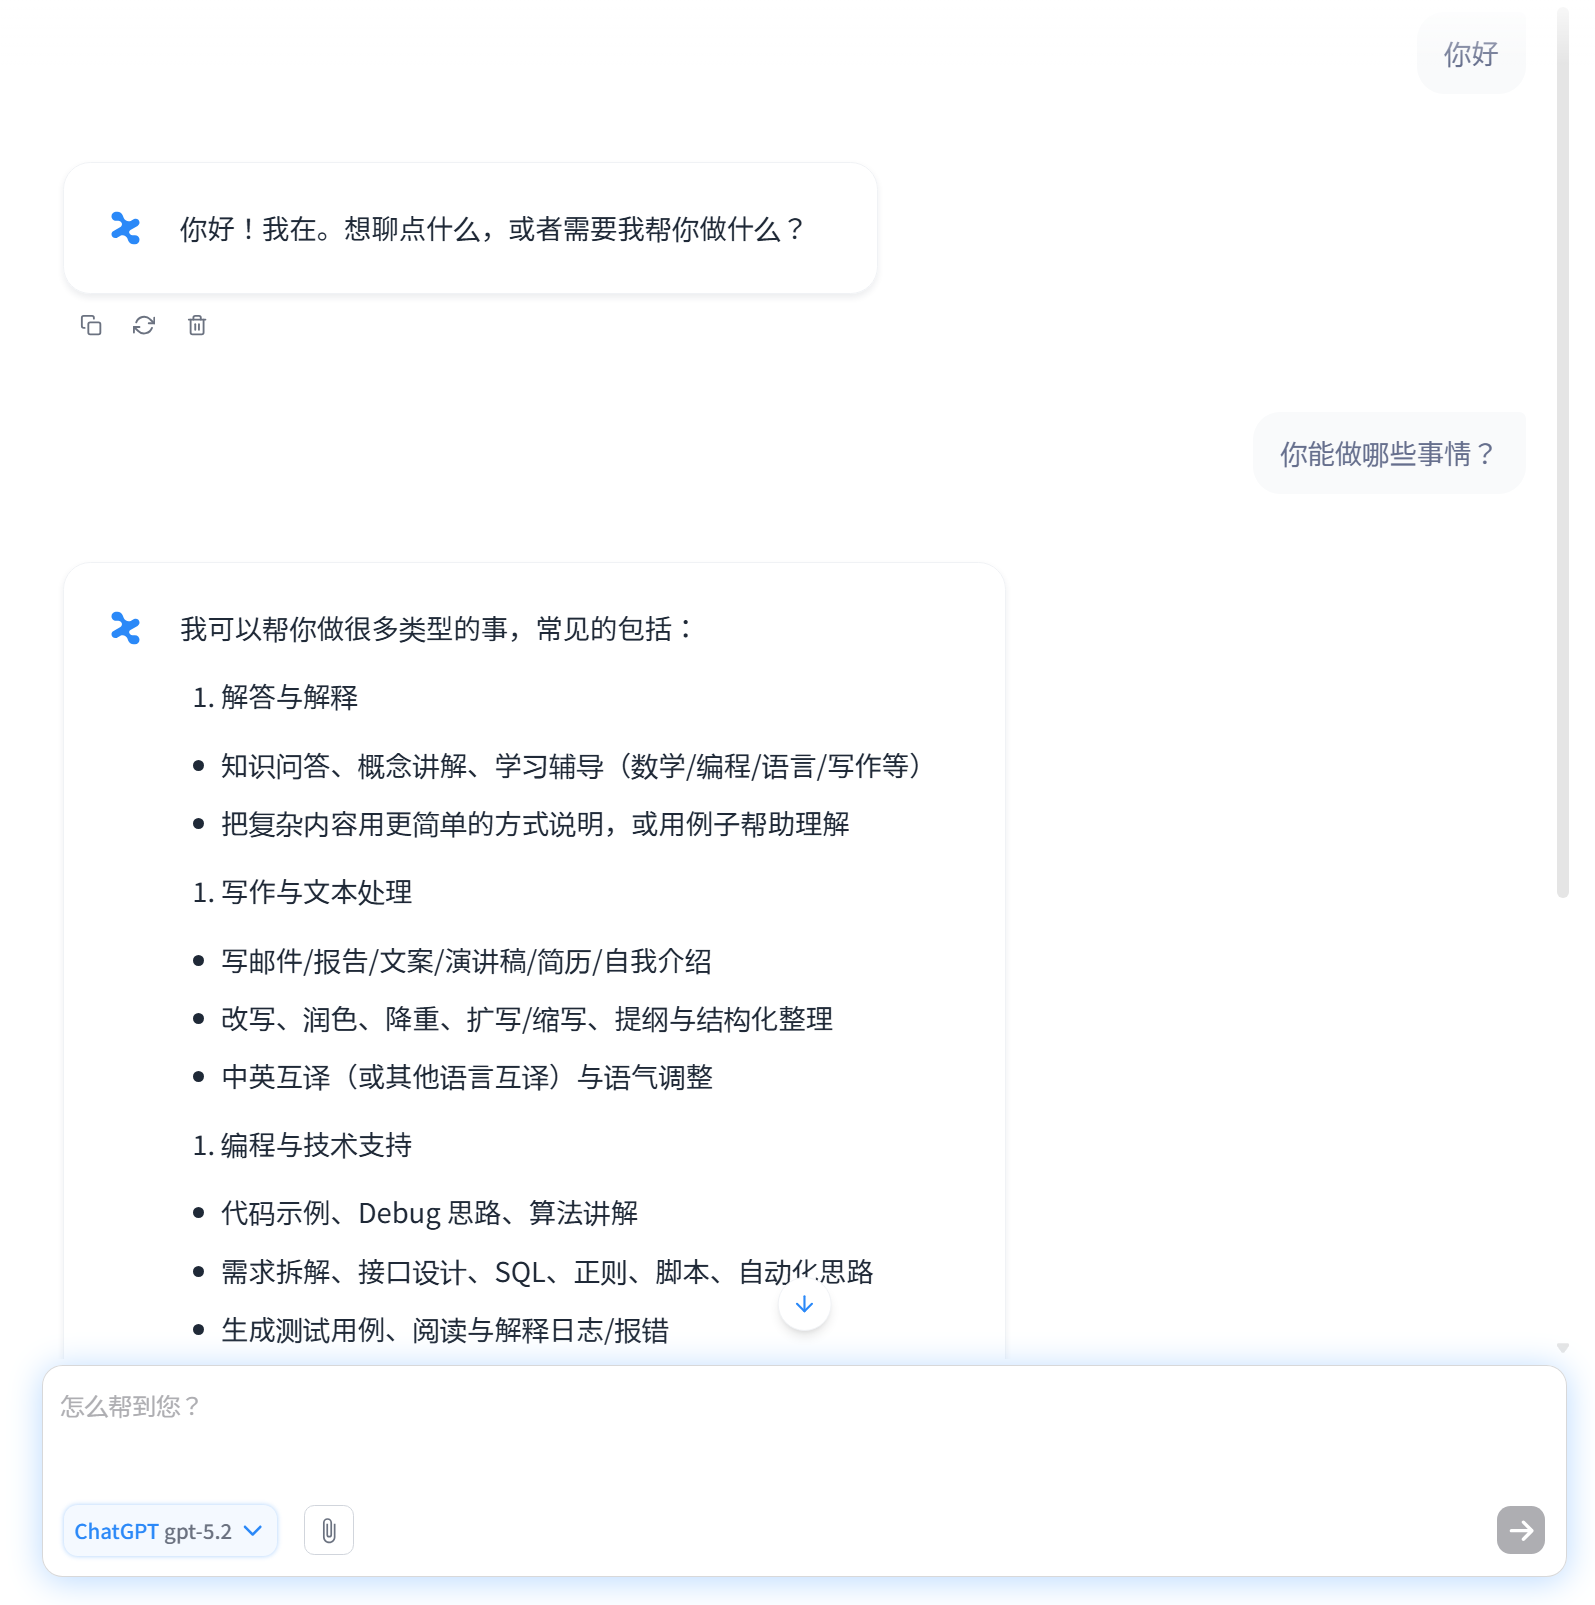
\includegraphics[width=\linewidth, height=12cm, keepaspectratio]{ai_conversation.png}\\[-0.1cm]
{\fontsize{22pt}{28pt}\selectfont 内置 AI 对话}
\end{minipage}\\[0.4cm]

\noindent
\begin{minipage}[t]{0.495\linewidth}\vspace{0pt}\centering
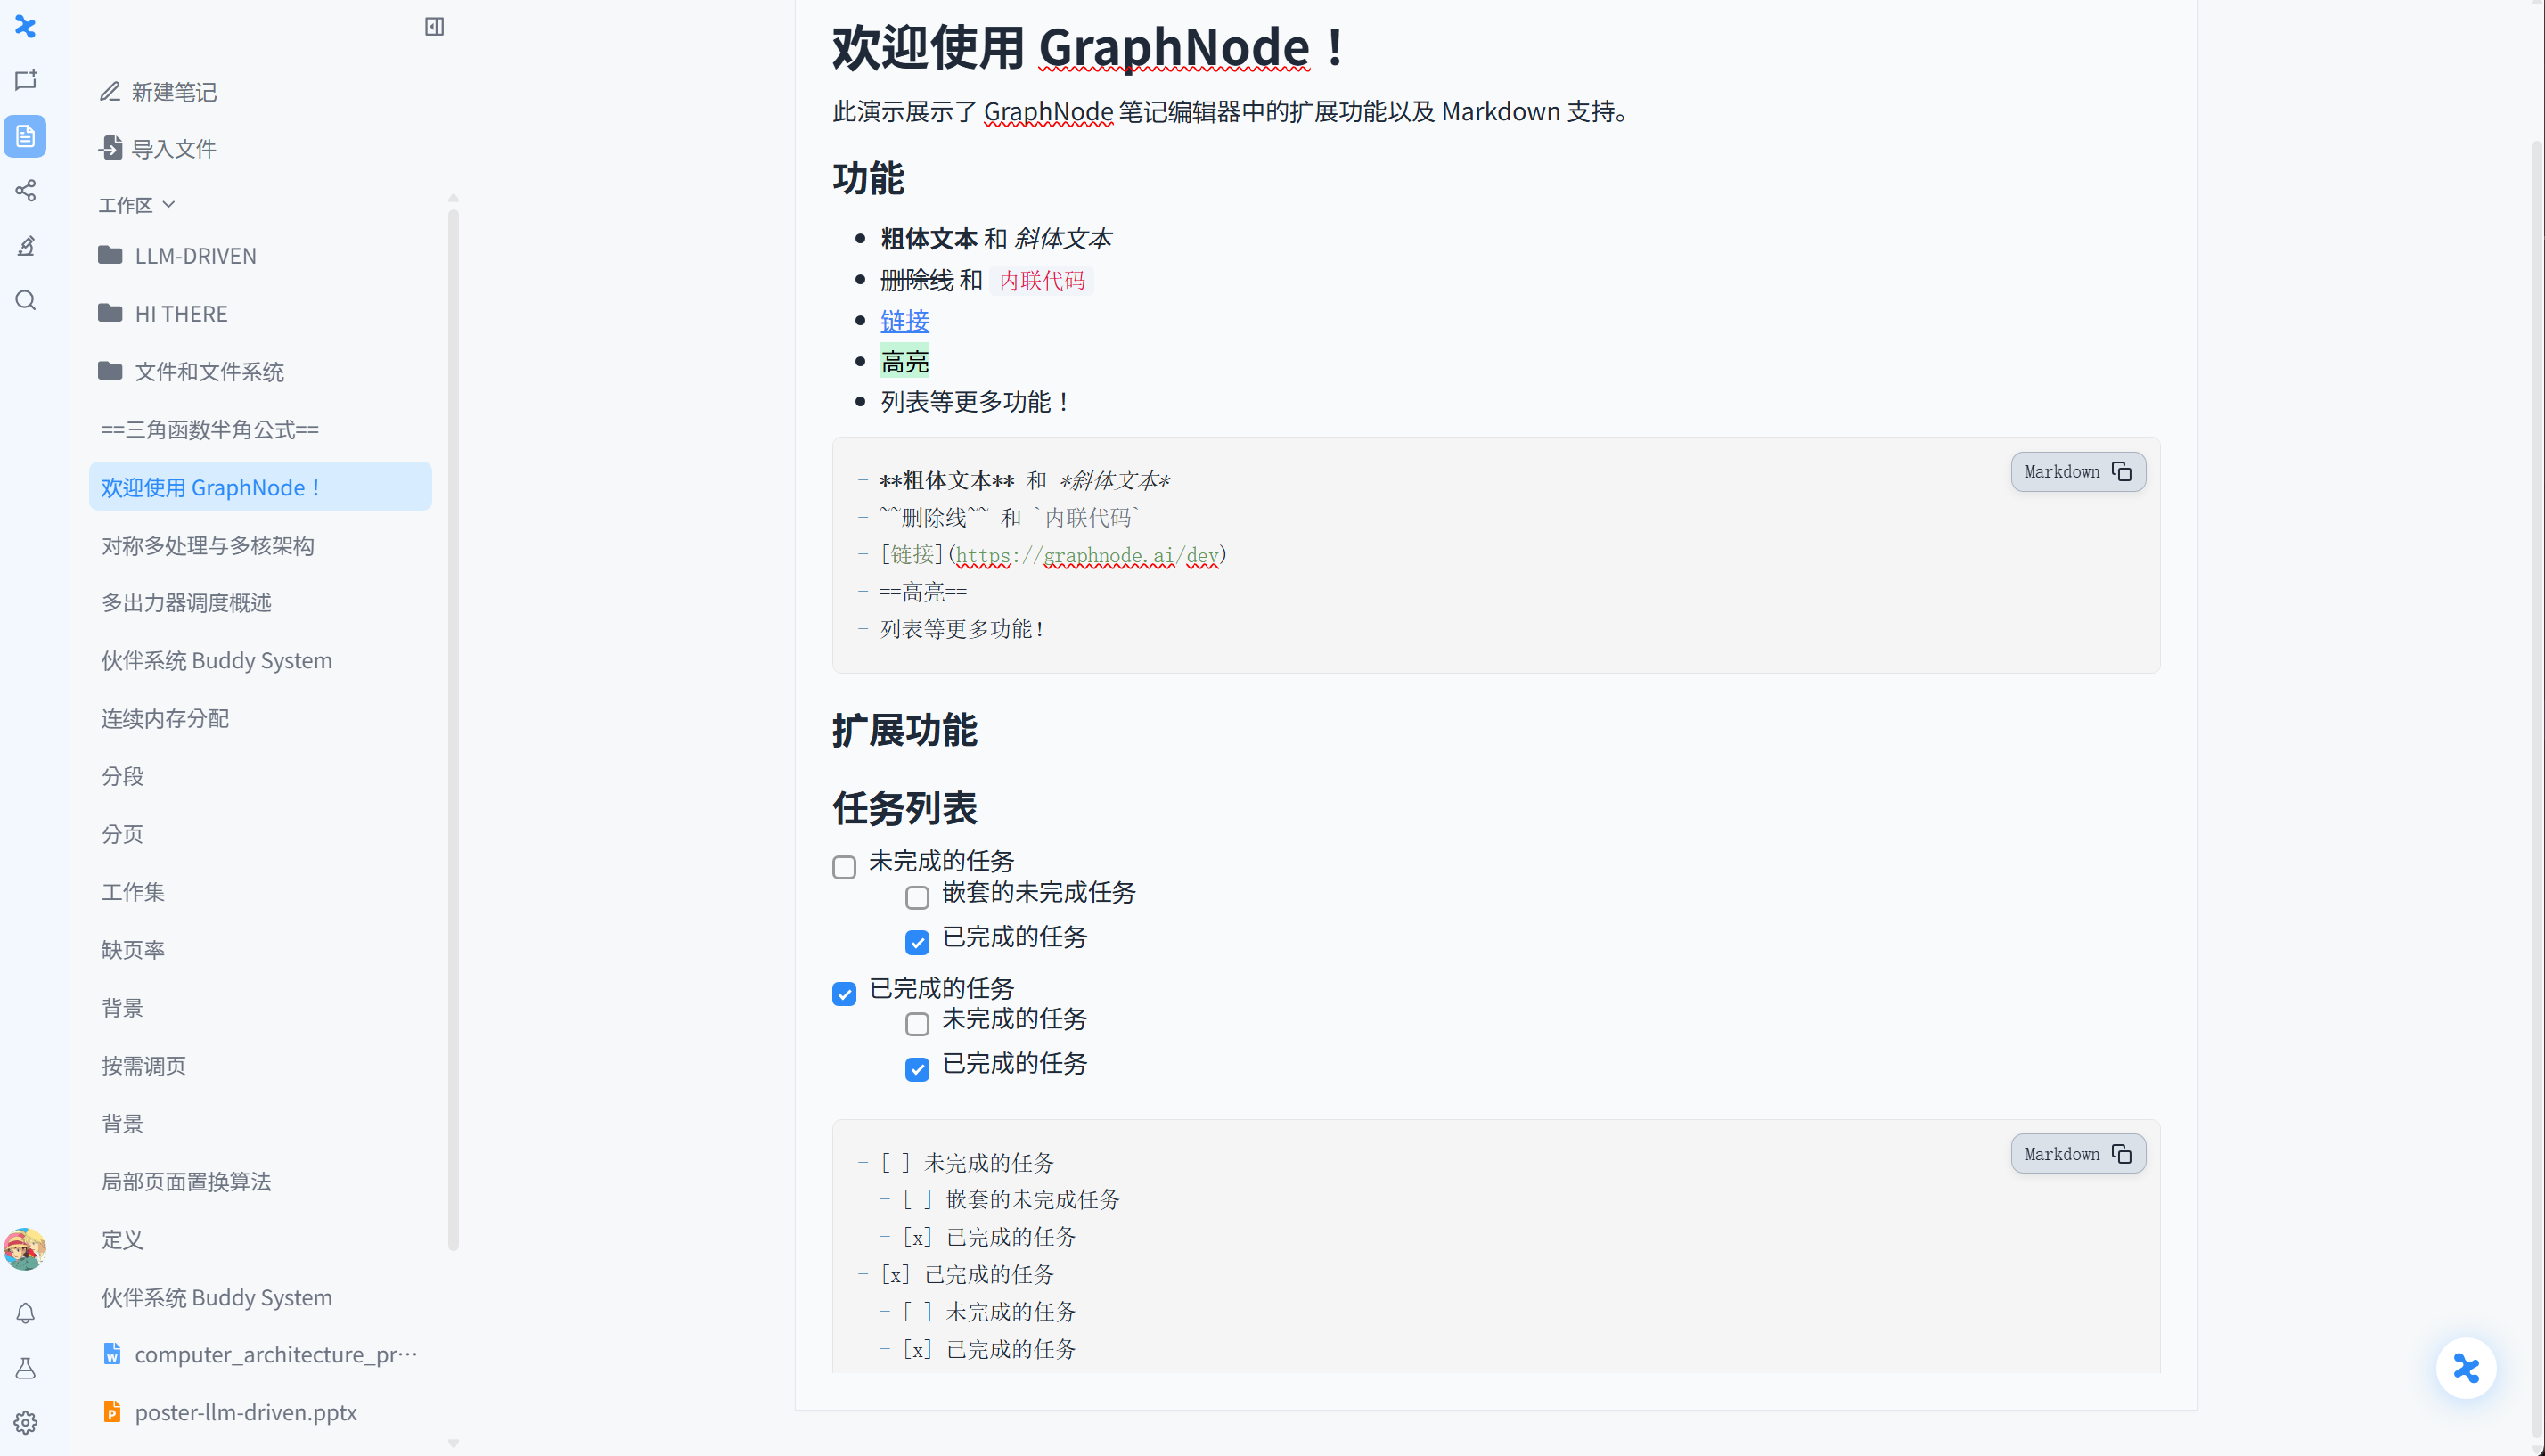
\includegraphics[width=\linewidth, height=12cm, keepaspectratio]{graphnode_note.png}\\[-0.1cm]
{\fontsize{22pt}{28pt}\selectfont 笔记编辑器}
\end{minipage}\hfill
\begin{minipage}[t]{0.495\linewidth}\vspace{0pt}\centering
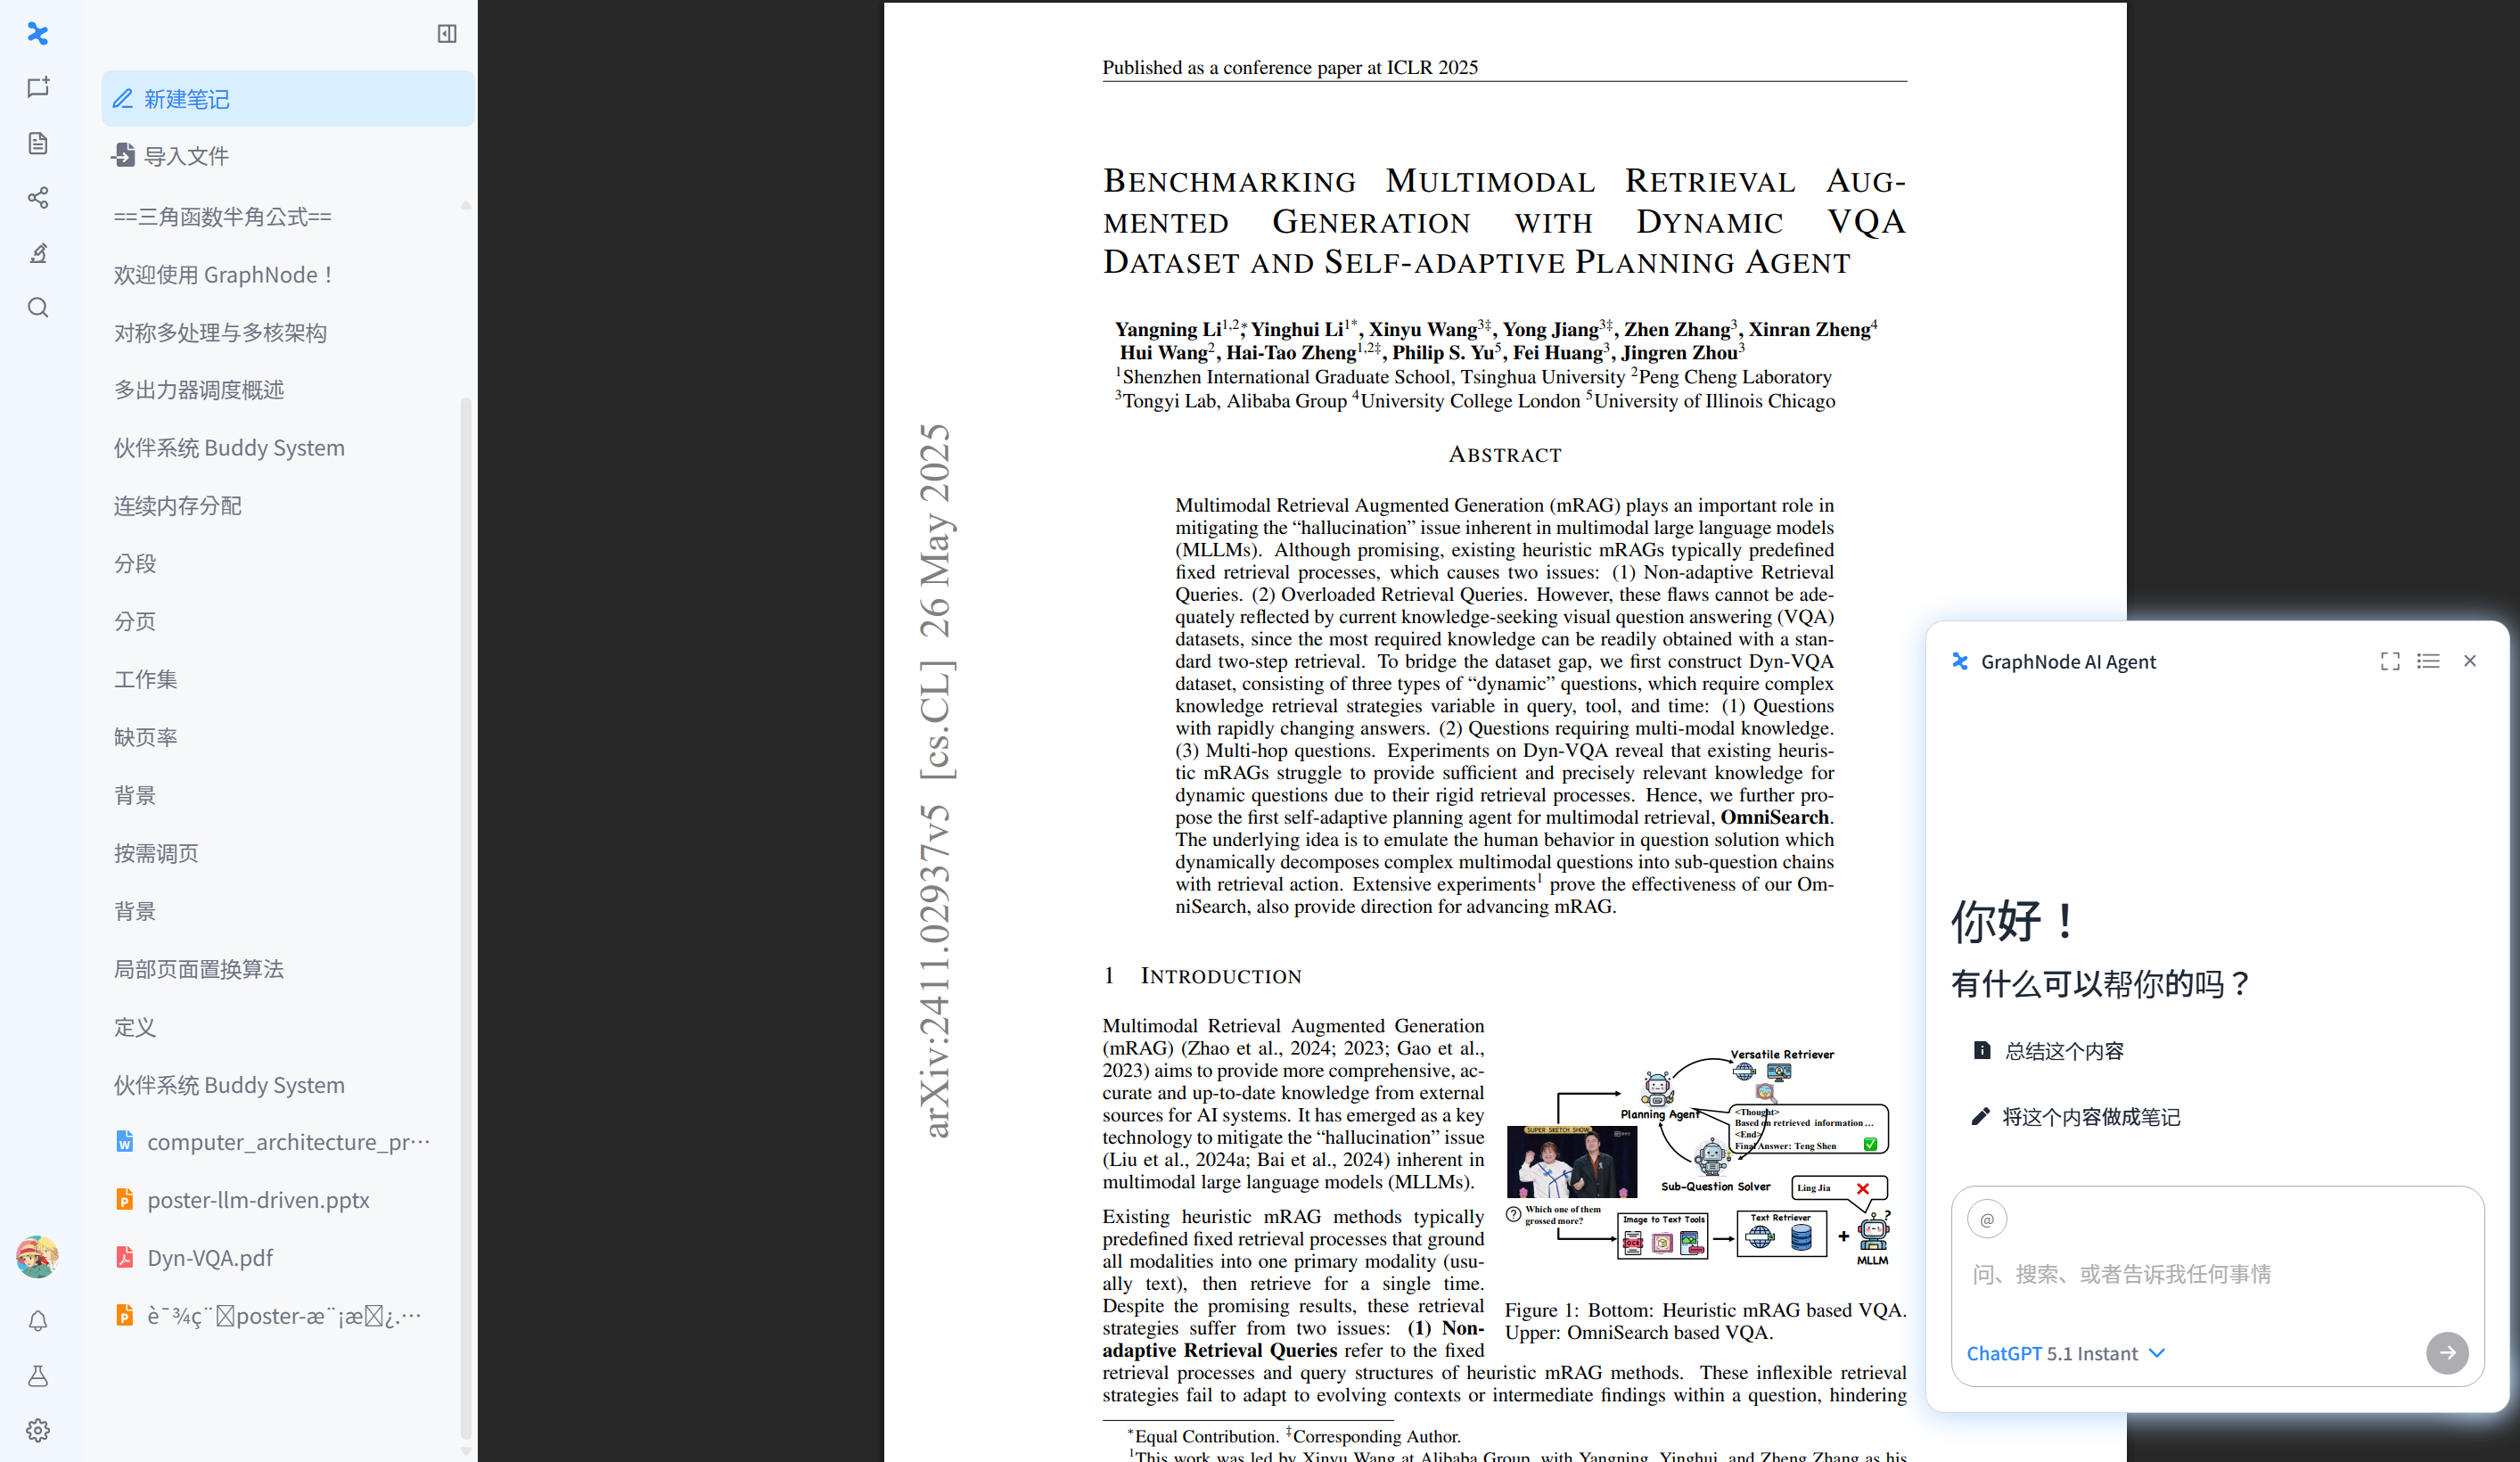
\includegraphics[width=\linewidth, height=12cm, keepaspectratio]{pdf_viewr_with_agent.png}\\[-0.1cm]
{\fontsize{22pt}{28pt}\selectfont 支持 docx / pdf/ pptx 等多种格式文档查看}
\end{minipage}
\end{block}

% ---- 5. 应用场景 Use Cases ----
\begin{block}{5. 应用场景 Use Cases}
\centering
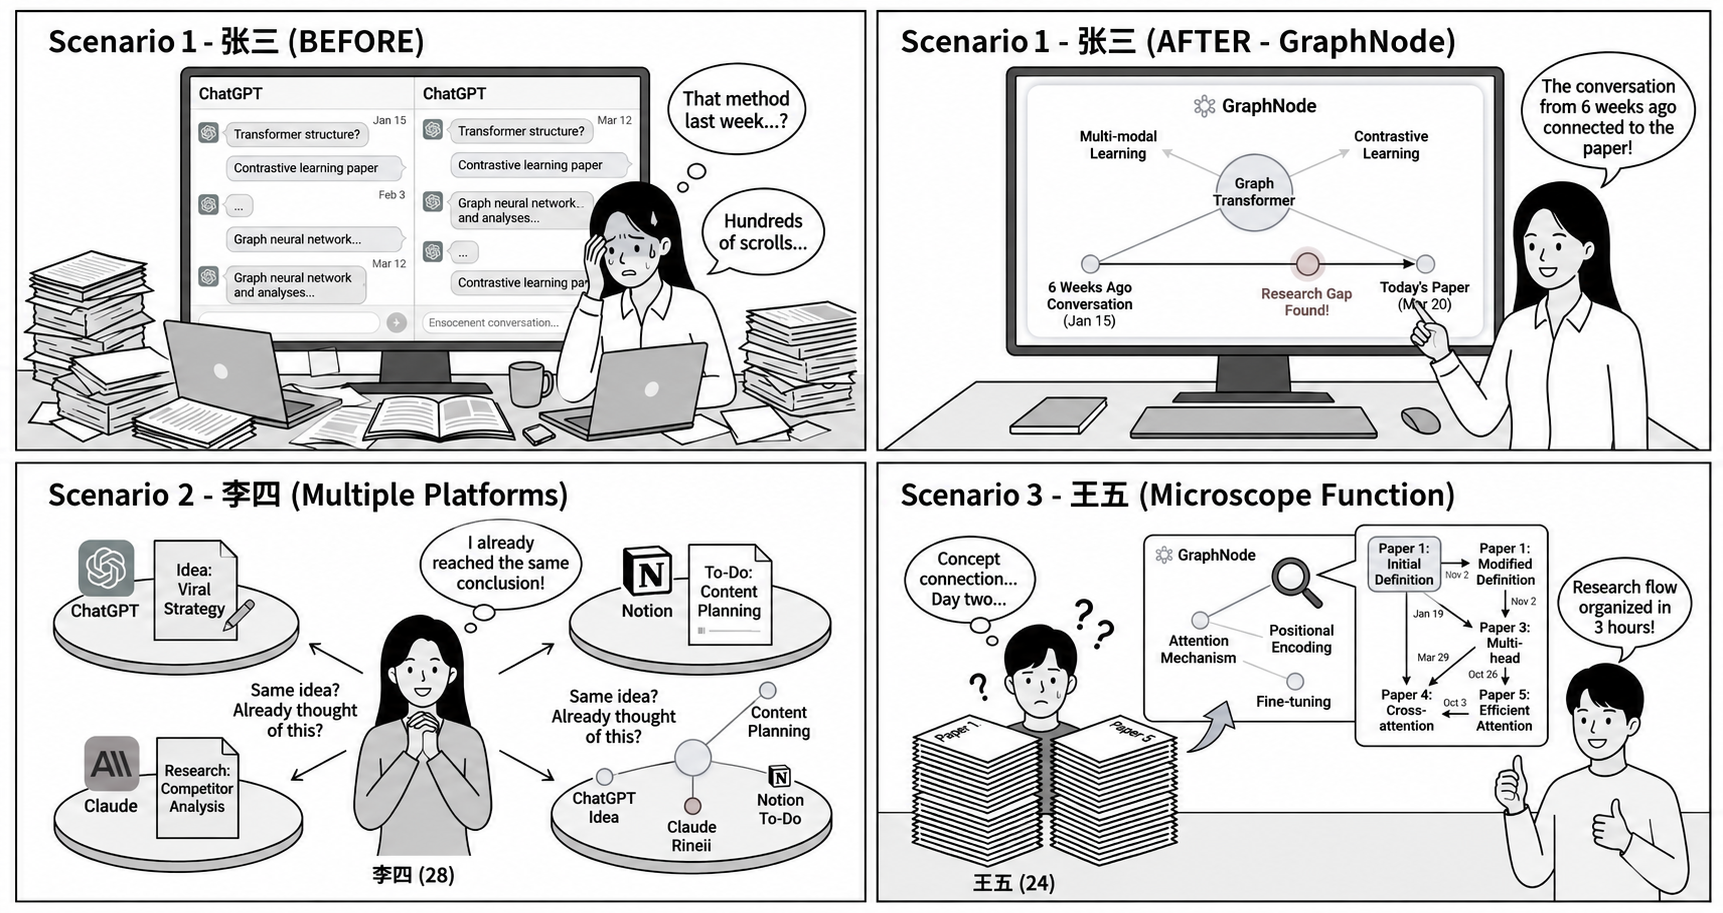
\includegraphics[width=0.95\linewidth, height=13cm, keepaspectratio]{usecase.jpg}\\[0.2cm]
\raggedright
\begin{itemize}
    \item \textbf{场景一 — 跨时间连接（缝合知识断层）}：自动将“6周前的历史灵感”与“今天的文献”建立图谱连线，精准找回上下文语境。
    \item \textbf{场景二 — 跨平台整合（打破信息孤岛）}：无缝接入 ChatGPT、Claude 与 Notion，将散落各处的同源想法统一聚合为单一知识网络。
    \item \textbf{场景三 — Microscope 深度解析（重塑研究脉络）}：将繁杂的课程笔记与文献，在极短时间内自动结构化，直观呈现概念的演进与逻辑。
\end{itemize}
\end{block}

% ---- 6. LLM 应用场景 ----
\begin{block}{6. LLM 应用场景}
\textbf{LLM 作为“知识结构化引擎”驱动整个软件。}\\[0.3cm]
\centering
{\fontsize{28pt}{38pt}\selectfont
\begin{tabular}{l|l}
\toprule
\textbf{功能} & \textbf{LLM 角色} \\
\midrule
Macro Graph 生成 & 主题分析、关键词提取、聚类标注 \\
Graph Summary   & 分析整体模式并提炼洞察 \\
Micro Graph 生成 & 提取单篇文档的概念-关系 \\
Agent Chat      & 以 Macro / Micro 模块为上下文问答 \\
\bottomrule
\end{tabular}}\\[0.15cm]
\end{block}

% ---- 7. 项目现状 & 未来路线图 ----
\begin{block}{7. 项目现状 \& 未来路线}
\textbf{三大核心机制}：
\begin{itemize}
    \item \textbf{跨平台整合}：打破时间与应用的壁垒，构建统一知识底座
    \item \textbf{Macro / Micro 双重视角}：全局俯瞰与单篇深挖相结合，自动生成图谱
    \item \textbf{GraphNode Agent}：基于动态图谱的精准 RAG 交互
\end{itemize}
\vspace{0.2cm}
\textbf{未来发展方向}：
\begin{itemize}
    \item \textbf{Agent 升级为“Pace-maker”}：深度结合用户当前目标（如备考、考研、面试准备），提供主动式陪伴与学习进度导航；
    \item \textbf{生态系统扩充}：在已跑通 \textbf{Notion} 同步的基础上，进一步深度接入 \textbf{Obsidian、飞书} 等主流生产力工具；
    \item \textbf{多模态知识解析}：突破纯文本限制，引入课程录像、会议语音等多模态数据的自动解析与图谱化支持。
\end{itemize}
\end{block}

\end{column}
\end{columns}

\end{frame}
\end{document}
